%% BioMed_Central_Tex_Template_v1.06
%%                                      %
%  bmc_article.tex            ver: 1.06 %
%                                       %

%%IMPORTANT: do not delete the first line of this template
%%It must be present to enable the BMC Submission system to
%%recognise this template!!

%%%%%%%%%%%%%%%%%%%%%%%%%%%%%%%%%%%%%%%%%
%%                                     %%
%%  LaTeX template for BioMed Central  %%
%%     journal article submissions     %%
%%                                     %%
%%          <8 June 2012>              %%
%%                                     %%
%%                                     %%
%%%%%%%%%%%%%%%%%%%%%%%%%%%%%%%%%%%%%%%%%


%%%%%%%%%%%%%%%%%%%%%%%%%%%%%%%%%%%%%%%%%%%%%%%%%%%%%%%%%%%%%%%%%%%%%
%%                                                                 %%
%% For instructions on how to fill out this Tex template           %%
%% document please refer to Readme.html and the instructions for   %%
%% authors page on the biomed central website                      %%
%% http://www.biomedcentral.com/info/authors/                      %%
%%                                                                 %%
%% Please do not use \input{...} to include other tex files.       %%
%% Submit your LaTeX manuscript as one .tex document.              %%
%%                                                                 %%
%% All additional figures and files should be attached             %%
%% separately and not embedded in the \TeX\ document itself.       %%
%%                                                                 %%
%% BioMed Central currently use the MikTex distribution of         %%
%% TeX for Windows) of TeX and LaTeX.  This is available from      %%
%% http://www.miktex.org                                           %%
%%                                                                 %%
%%%%%%%%%%%%%%%%%%%%%%%%%%%%%%%%%%%%%%%%%%%%%%%%%%%%%%%%%%%%%%%%%%%%%

%%% additional documentclass options:
%  [doublespacing]
%  [linenumbers]   - put the line numbers on margins

%%% loading packages, author definitions

%\documentclass[twocolumn]{bmcart}% uncomment this for twocolumn layout and comment line below
\documentclass{bmcart}

%%% Load packages
%\usepackage{amsthm,amsmath}
%\RequirePackage{natbib}
%\RequirePackage[authoryear]{natbib}% uncomment this for author-year bibliography
%\RequirePackage{hyperref}
\usepackage[utf8]{inputenc} %unicode support
%\usepackage[applemac]{inputenc} %applemac support if unicode package fails
%\usepackage[latin1]{inputenc} %UNIX support if unicode package fails
\usepackage{graphicx} 
\usepackage{xspace}


%%%%%%%%%%%%%%%%%%%%%%%%%%%%%%%%%%%%%%%%%%%%%%%%%
%%                                             %%
%%  If you wish to display your graphics for   %%
%%  your own use using includegraphic or       %%
%%  includegraphics, then comment out the      %%
%%  following two lines of code.               %%
%%  NB: These line *must* be included when     %%
%%  submitting to BMC.                         %%
%%  All figure files must be submitted as      %%
%%  separate graphics through the BMC          %%
%%  submission process, not included in the    %%
%%  submitted article.                         %%
%%                                             %%
%%%%%%%%%%%%%%%%%%%%%%%%%%%%%%%%%%%%%%%%%%%%%%%%%


%\def\includegraphic{}
%\def\includegraphics{}



%%% Put your definitions there:
\startlocaldefs
\def\OpBook {Open-Book view\xspace}
\def\ExpView {Exploded view\xspace}
\def\MatView {Matrix view\xspace}
\def\CoZoListView {Contact-Zone list-view\xspace}
\def\CoZoList{Contact-Zone list\xspace}
\def\CoZoLists{Contact-Zone lists\xspace}

\endlocaldefs


%%% Begin ...
\begin{document}

%%% Start of article front matter
\begin{frontmatter}

\begin{fmbox}
\dochead{Research}

%%%%%%%%%%%%%%%%%%%%%%%%%%%%%%%%%%%%%%%%%%%%%%
%%                                          %%
%% Enter the title of your article here     %%
%%                                          %%
%%%%%%%%%%%%%%%%%%%%%%%%%%%%%%%%%%%%%%%%%%%%%%

\title{COZOID: COntact ZOne IDentifier for Visual Analysis of Protein-Protein Interactions}

%%%%%%%%%%%%%%%%%%%%%%%%%%%%%%%%%%%%%%%%%%%%%%
%%                                          %%
%% Enter the authors here                   %%
%%                                          %%
%% Specify information, if available,       %%
%% in the form:                             %%
%%   <key>={<id1>,<id2>}                    %%
%%   <key>=                                 %%
%% Comment or delete the keys which are     %%
%% not used. Repeat \author command as much %%
%% as required.                             %%
%%                                          %%
%%%%%%%%%%%%%%%%%%%%%%%%%%%%%%%%%%%%%%%%%%%%%%
\author[
   addressref={aff1},
   email={furmanova@mail.muni.cz}
]{\inits{KF}\fnm{Katar\'{i}na} \snm{Furmanov\'{a}}}
\author[
   addressref={aff2},     % id's of addresses, e.g. {aff1,aff2}
   email={jan.byska@gmail.com}   % email address
]{\inits{JB}\fnm{Jan} \snm{By\v{s}ka}}
\author[
   addressref={aff3},             % id's of addresses, e.g. {aff1,aff2}
   email={groeller@cg.tuwien.ac.at}   % email address
]{\inits{EMG}\fnm{Eduard M} \snm{Gr\"{o}ller}}
\author[
   addressref={aff3},             % id's of addresses, e.g. {aff1,aff2}
   email={viola@cg.tuwien.ac.at}   % email address
]{\inits{IV}\fnm{Ivan} \snm{Viola}}
\author[
   addressref={aff4, aff5},             % id's of addresses, e.g. {aff1,aff2}
   email={jpalecek@sci.muni.cz}   % email address
]{\inits{JJP}\fnm{Jan J} \snm{Pale\v{c}ek}}
\author[
   addressref={aff1},             % id's of addresses, e.g. {aff1,aff2}
   corref={aff1},
   email={kozlikova@fi.muni.cz}   % email address
]{\inits{BK}\fnm{Barbora} \snm{Kozl\'{i}kov\'{a}}}

%%%%%%%%%%%%%%%%%%%%%%%%%%%%%%%%%%%%%%%%%%%%%%
%%                                          %%
%% Enter the authors' addresses here        %%
%%                                          %%
%% Repeat \address commands as much as      %%
%% required.                                %%
%%                                          %%
%%%%%%%%%%%%%%%%%%%%%%%%%%%%%%%%%%%%%%%%%%%%%%

\address[id=aff1]{%                           % unique id
  \orgname{Faculty of Informatics, Masaryk University}, % university, etc
 % \street{\v{Z}erot\'{i}novo n\'{a}m\v{e}st\'{i}},                     %
  %\postcode{}                                % post or zip code
  \city{Brno},                              % city
  \cny{Czech Republic}                                    % country
}
\address[id=aff2]{%
  \orgname{Department of Informatics, University of Bergen},
  %\street{D\"{u}sternbrooker Weg 20},
  %\postcode{24105}
  \city{Bergen},
  \cny{Norway}
}
\address[id=aff3]{%
  \orgname{Institute of Computer Graphics and Algorithms, TU Wien},
  %\street{D\"{u}sternbrooker Weg 20},
  %\postcode{24105}
  \city{Wien},
  \cny{Austria}
}

\address[id=aff4]{%                           % unique id
  \orgname{National Centre for Biomolecular Research, Masaryk University}, % university, etc
 % \street{\v{Z}erot\'{i}novo n\'{a}m\v{e}st\'{i}},                     %
  %\postcode{}                                % post or zip code
  \city{Brno},                              % city
  \cny{Czech Republic}                                    % country
}

\address[id=aff5]{%                           % unique id
  \orgname{Central European Institute of Technology, Masaryk University}, % university, etc
 % \street{\v{Z}erot\'{i}novo n\'{a}m\v{e}st\'{i}},                     %
  %\postcode{}                                % post or zip code
  \city{Brno},                              % city
  \cny{Czech Republic}                                    % country
}


%%%%%%%%%%%%%%%%%%%%%%%%%%%%%%%%%%%%%%%%%%%%%%
%%                                          %%
%% Enter short notes here                   %%
%%                                          %%
%% Short notes will be after addresses      %%
%% on first page.                           %%
%%                                          %%
%%%%%%%%%%%%%%%%%%%%%%%%%%%%%%%%%%%%%%%%%%%%%%

%\begin{artnotes}
%\note{Sample of title note}     % note to the article
%\note[id=n1]{Equal contributor} % note, connected to author
%\end{artnotes}

\end{fmbox}% comment this for two column layout

%%%%%%%%%%%%%%%%%%%%%%%%%%%%%%%%%%%%%%%%%%%%%%
%%                                          %%
%% The Abstract begins here                 %%
%%                                          %%
%% Please refer to the Instructions for     %%
%% authors on http://www.biomedcentral.com  %%
%% and include the section headings         %%
%% accordingly for your article type.       %%
%%                                          %%
%%%%%%%%%%%%%%%%%%%%%%%%%%%%%%%%%%%%%%%%%%%%%%

\begin{abstractbox}

\begin{abstract} % abstract
\parttitle{Background} %if any
Studying the patterns of protein-protein interactions (PPIs) is fundamental for understanding the structure and function of protein complexes. 
The exploration of the vast space of possible mutual configurations of interacting proteins and their contact zones is very time consuming and requires the proteomic expert knowledge.
\parttitle{Results}
In this paper, we propose a novel tool contaning a set of visual abstraction techniques for a guided exploration of the PPI configuration space.
It helps the proteomic experts to select the most relevant configurations and explore their contact zones on different levels of detail. 
The system integrates a set of methods following and supporting the workflow of proteomics experts. 
The first visual abstraction method, the Matrix view, is based on customized interactive heat maps and provides the users with an overview of all possible residue-residue contacts in all PPI configurations and their interactive filtering. 
In this step, the user can traverse all input PPI configurations and gets an overview of their interacting amino acids.
Then, the models containing a particular pair of interacting amino acids can be selectively picked and traversed. 
The detailed information about individual amino acids in the contact zones and their properties is presented by the Contact-Zone list-view. 
The list-view provides a comparative tool to rank the best models based on the similarity of their contacts to the template-structure contacts. 
All these techniques are interactively linked with another proposed methods, the Exploded view and the Open-Book view, that represent individual configurations in the three-dimensional space. 
These representations solve the problem of high overlaps of many configurations. 
Using these views, the structural alignment of the best models can be visually confirmed as well.
\parttitle{Conclusions}
We developed a system for the exploration of large sets of protein-protein complexes in a fast and intuitive way. The usefulness of our system has been tested and verified on several docking structures, covering three major types of PPIs, i.e, coiled-coil, pocket-string, and surface-surface interactions. Our case studies prove, that our tool helps to analyze and filter protein-protein complexes in a fraction of time spent when using the previously available techniques.
\end{abstract}

%%%%%%%%%%%%%%%%%%%%%%%%%%%%%%%%%%%%%%%%%%%%%%
%%                                          %%
%% The keywords begin here                  %%
%%                                          %%
%% Put each keyword in separate \kwd{}.     %%
%%                                          %%
%%%%%%%%%%%%%%%%%%%%%%%%%%%%%%%%%%%%%%%%%%%%%%

\begin{keyword}
\kwd{protein-protein interaction}
\kwd{contact zone}
\kwd{visualization}
\end{keyword}

% MSC classifications codes, if any
%\begin{keyword}[class=AMS]
%\kwd[Primary ]{}
%\kwd{}
%\kwd[; secondary ]{}
%\end{keyword}

\end{abstractbox}
%
%\end{fmbox}% uncomment this for twcolumn layout

\end{frontmatter}

%%%%%%%%%%%%%%%%%%%%%%%%%%%%%%%%%%%%%%%%%%%%%%
%%                                          %%
%% The Main Body begins here                %%
%%                                          %%
%% Please refer to the instructions for     %%
%% authors on:                              %%
%% http://www.biomedcentral.com/info/authors%%
%% and include the section headings         %%
%% accordingly for your article type.       %%
%%                                          %%
%% See the Results and Discussion section   %%
%% for details on how to create sub-sections%%
%%                                          %%
%% use \cite{...} to cite references        %%
%%  \cite{koon} and                         %%
%%  \cite{oreg,khar,zvai,xjon,schn,pond}    %%
%%  \nocite{smith,marg,hunn,advi,koha,mouse}%%
%%                                          %%
%%%%%%%%%%%%%%%%%%%%%%%%%%%%%%%%%%%%%%%%%%%%%%

%%%%%%%%%%%%%%%%%%%%%%%%% start of article main body
% <put your article body there>

%%%%%%%%%%%%%%%%
%% Background %%
%%
\section*{Background}
Understanding the constitution and biological function of proteins is essential in many research disciplines, such as medicine and pharmaceutics.
%This knowledge is tightly connected with the ability of the protein to interact with other molecules.
Most of the proteins critical for the cellular life act in a cooperative manner, forming multiprotein complexes. 
It is estimated that about 800 complexes exist in just one yeast cell~\cite{Gavin}. 

All complexes are composed of subunits, which constitute the complex via mutual protein-protein interactions (PPIs).
The main goal of the process of studying such PPIs, known as protein-protein docking, is to identify an appropriate spatial \textbf{configuration} of the interacting proteins.
Such a configuration is represented by the mutual spatial orientation of the interacting proteins.
Each configuration contains a \textbf{contact zone}, consisting of the set of amino acids from both interacting proteins that are in the interaction distance, usually spanning from 3 to 5 \AA ngstr\"{o}ms.
%These thresholds are commonly used by the existing computational tools, but can be customized by users.
%In other words, the contact zone resides on the interface between the interacting proteins and is formed by mutually interacting amino acids.

The structure determination of PPIs in laboratories is very challenging as well as expensive and time consuming.
This is due to many problems related to the dynamic nature of the proteins, the difficulties with their purification and the preparation of samples.
Therefore, the computational docking is often used to study the feasibility of proposed configurations.
Many algorithms and tools have appeared in this respect in the last years.
A categorization of the existing algorithms, along with the description of their basic principles, was published recently by Huang~\cite{Huang2014}.
%However, these algorithms produce a large number of possible configurations.
%The domain expert has to explore them and select the biochemically most relevant ones. 
However, these algorithms produce a large number of possible configurations, which need to be explored to identify the proteomically most relevant ones.
Even though the computational tools usually provide the users with some score to rank the configurations, the resulting ordering mostly does not correspond to their proteomical relevance.
Therefore, the configurations have to be processed and examined manually, which requires a proper visual support to enhance the exploration process.

It is obvious that even for the comparison of two configurations, the traditional overlay representation suffers from many occlusion problems and it is hard to perceive the differences between individual solutions.
When comparing more configurations, even without a detailed visualization of the hot spot amino acids, the problem becomes even more apparent (Figure~\ref{fig:problem}).


\subsection*{Related Work}
As the selection of the most proteomically relevant PPI configurations is a very challenging task, several algorithms have already been published for re-ranking of the configurations according to different criteria.
They suggest a subset of configurations that should be explored in detail.
As a representative of these attempts, Malhotra et al.~\cite{Malhotra2015} presented DockScore, a webserver for ranking the individual configurations produced by the docking tools. 
Their idea is based on building a scoring scheme considering several interface parameters, such as the surface area, hydrophobicity, spatial clustering, etc.
This helps the user to reduce the number of configurations to a smaller set, which still has to be explored manually.
For this exploration, a visual support is essential, as it enables the user to see the spatial orientation of the contact zones and to compare different configurations.
However, DockScore provides only a rudimentary visual representation of top five configurations, which is insufficient for the proper exploration of the configuration space.
 
The issue of finding a proper visual representation of PPIs can be tackled from different perspectives. One group consists of techniques visualizing the contact zones and their interacting amino acids.
The spatial techniques have to deal with the problem of occlusion and visual clutter caused by the fact that the most interesting parts of the interacting proteins, the contact zones, are facing each other inside the configuration.
Without transformations or visual enhancements (e.g., through transparency) it is impossible to visually explore the contact zones.
Jin et al.~\cite{Jin2014} presented an open-book view where the interacting proteins are rotated to orient the contact zones towards the camera.
The problem of the presented solution lies mainly in the missing information about the interacting amino acids and the unified coloring of the contact zones.
An alternative approach presented by Lee and Varshney~\cite{Varshney2003} computes and visualizes the intermolecular negative volume and the area of the docking site. %(Figure~\ref{fig:varshney}b,c).
This way, the users can observe the volume between the interacting proteins without the necessity to display the contact zones themselves.
This can serve the proteomic experts as an interactive tool for studying possible docking configurations but it does not support their comparison.
Similar approaches suggest the construction of interface surface between the interacting proteins~\cite{480793, Ban2006}.
The surface is visualized as a 3D mesh, encoding the information about the core and peripheral regions of the interface. 
However, this method also does not support the comparison of multiple configurations.

%One of our proposed spatial visualizations adapts the idea of the exploded view.
%This technique also enables the observation of the parts of objects, which are originally hidden, by enlarging their mutual distance.
%Bruckner et al.~\cite{Bruckner2006} applied this technique to volume data and demonstrated it on the scans of different parts of human body.

Two-dimensional abstract representations are also commonly used for the visualization of contact zones, such as the schematic representation used by the PDBsum database~\cite{pdbsum} (Figure~\ref{fig:pdbsum}).
In the overview visualization, each of the interacting proteins is represented by a circle equipped with the information about the number of amino acids forming the contact zones and the number of different types of interactions in-between (e.g., salt bridges, disulphide bonds, hydrogen bonds, or non-bonded contacts).
The detailed visualization in the PDBsum lists all contact-zone amino acids. 
The interactions are visualized by lines of different colors and thickness, which represent the type and strength of the interactions, respectively. 
This approach gives a comprehensible overview of one configuration, but comparing it with another configuration is not possible.

%Abstracted representations have been already successfully applied to protein-ligand docking.
%LigPlot+~\cite{laskowski2011ligplot+} is an interactive system for generating 2D protein-ligand interaction diagrams. 
%In this tool, a flattened 2D representation of a ligand is placed at the center of the diagram and the interacting protein residues are positioned around it at the corresponding positions. 
%Superimposition can be used to compare multiple diagrams, i.e., when multiple ligands bind to the same protein or one ligand binds to several homologous proteins. 
%However, this approach is suitable only for small ligand molecules, consisting of several atoms, thus it is not applicable to PPIs.

%Byska et al.~\cite{Byska2015} proposed visual abstractions of protein tunnels serving ligand transportation and their evolution in molecular dynamics simulations.
%Their ATH and STH representations show heat maps encoding the information about tunnel openness over time.
%The MoleCollar visualization depicts the evolution of the shape of the narrowest tunnel part, i.e., its bottleneck.
%The visualization contains also the information about the position and a set of physico-chemical properties of amino acids surrounding the tunnel bottleneck.

Lex et al.~\cite{Lex2012} proposed a visual analysis tool serving for the exploration of large-scale heterogeneous genomics data for the characterization of cancer subtypes.
They use multiple views of the complex data and one of them is a method for the comparison of different datasets.
The abstracted representation shows the similarities in the datasets by connecting the corresponding blocks of data. 
The thickness of a connection denotes the degree of similarity. 
This representation serves well for the comparison but it lacks the detailed information about individual items.
%This representation is to some extent similar to our proposed InCo lens view, but in our case we primarily focus on the exploration of the interacting amino acids in individual configurations.

%In one of our proposed methods, the \MatView, we tackle the problem of visualizing many items in a limited 2D space.
%This may lead to having only little space available for individual items, which are then hard to perceive.
%Therefore, we also had to adapt one of the interactive lens techniques, which were thoroughly surveyed by Tominski et al.~\cite{Tominski2014}.

%In this paper we propose a solution to these problems.
In this paper, we present a systemic tool, COZOID (COntact ZOne IDentifier), comprised of a set of methods for the visualization, comparison, and selection of numerous docking configurations.
The combination of our proposed methods eliminates the problems of the existing solutions and provides the proteomic experts with an intuitive and user-friendly tool for the interactive exploration of PPIs.
Our tool is integrated into the CAVER Analyst software~\cite{kozlikova2014caver}, serving for analysis and visualization of biomolecules, thus containing many relevant features, such as different molecular visualization modes, measurement tools, etc.  
The input PPI configurations are provided by the existing computational tools and our solution is designed for dealing specifically with a large number of configurations.

\section*{Methods}
\subsection*{COZOID Overview}
Our newly proposed system enables the efficient visual exploration of a large number of PPI complexes.
For better understanding, we introduce the following notation.
A protein $P$ consists of a set of amino acids forming the polypeptidic chain.
A \textbf{complex} $C$ is represented by a set of mutually interacting proteins.
In our case, we focus primarily on interactions between two protein structures $P_1$ and $P_2$, determining a complex $C(P_1,P_2)$.
The mutual spatial orientation of the interacting proteins in the complex forms a \textbf{configuration}.
The $i$-th configuration of complex $C(P_1,P_2)$, denoted as $CONF_i(C(P_1,P_2))$, represents one of the possible mutual orientations of this complex.
Generally, there can be $n$ ($1 \leq i \leq n$) possible configurations for a given complex and the task is to select the configuration that is the most relevant one from a proteomical point of view.
The decision is based on various pieces of knowledge about the geometric arrangement of the configuration as well as other aspects, such as the knowledge of contacts between the amino acids present in the contact zone of the given configuration.
Therefore, the selection of the most relevant configurations cannot be done automatically and requires the insight of the proteomic expert.
Therefore, this represents a typical domain-related problem, which has to be supported by specifically designed visualizations.

The visualization methods proposed in this paper allow the user to visually explore a set of possible configurations detected by one of the existing computational tools and to select the proteomically most relevant ones.
The users have to iteratively filter out those configurations that do not fulfill the given specific criteria.
The workflow of the proteomic experts, along with our proposed visual support of its individual stages, is depicted in Figure~\ref{fig:workflow}.
The input datasets, consisting of dozens of configurations between two interacting proteins, were computed using the HADDOCK~\cite{haddock} and the PyDock~\cite{pydock} tools. 
However, any of the existing tools for protein-protein docking can serve as a source of input data for our system.

The proposed visualizations are based on the precondition that the users have already an initial knowledge about the interacting proteins.
Thus the experts are able to define a pair of amino acids which is expected to interact.
This is not restrictive as the computational tools also require this information in order to produce a meaningful set of configurations. 
In other words, we are using the similar input information as the computational tools.
The second possibility is that the users do not have such information but are aware of an already explored protein complex with similar structure, which can serve as a reference (primary) complex for further comparison and exploration. 
In this case the computational tools usually produce even more configurations, but most of them are irrelevant and have to be filtered out. 
Our tool can utilize the information about the interactions in the primary complex and thus enhances the filtering process.

Our methods have been designed specifically in order to help the proteomic experts to answer the following questions:
\begin{itemize}
\item Q1: Which configurations contain a selected interacting pair of amino acids (and what is the frequency of occurrence of this pair in all configurations)?
\item Q2: Which pairs of amino acids are present in a given configuration?
\item Q3: How close are the amino acids in the contact zone and which are the closest ones?
\item Q4: How similar and different are the contact zones in the configurations?
\item Q5: What are the physico-chemical properties of the amino acids in the contact zone?
%\item Q8: How exactly does the contact zone of a selected configuration look like? How is the correspondence between its amino acids?
\item Q6: What are the differences between the sets of amino acids in the contact zones of different configurations?
\end{itemize}

Answering these questions helps the proteomic experts to better understand the interactions in the protein-protein complexes and to evaluate the correctness of the given configurations.
The proposed visualizations enable to find the answers by interactively exploring the configurations.
In the following chapters, we introduce our proposed views in detail.

%%%%%%%%%%%%%%%%%%%%%%%%%%%%%%%%%%%%%%%%%%%%%%%%%%%%%%%%%%%%

\subsection*{Matrix View}
\label{sec:matview}
When using a computational tool for generating possible configurations, the resulting set $S = \{CONF_i(C(P_1,P_2)); 1 \leq i \leq n\}$, $n$ can be very large, ranging from dozens to hundreds. 
This amount is impossible to explore manually one-be-one, thus some preliminary filtering is crucial.
The filtering stage is designed to answer the question Q1.
We propose a matrix-based visualization inspired by commonly used heat maps (Figure~\ref{fig:matrixlens}a).
The rows and columns of the \MatView correspond to interacting proteins $P_1$ and $P_2$ respectively.
Each row or column represents one amino acid present in a contact zone of some of the configurations $CONF_i(C(P_1,P_2))$. 
The rows and columns are formed only by those amino acids from the interacting proteins which are in contact in at least one configuration.
The contact between the amino acids is based on their Euclidean distance. 
Two amino acids are considered to be in contact if their distance is between 3 and 5 \AA ngstr\"{o}ms.
This range can be interactively changed by the user.
The color of each cell in the matrix corresponds to the number of occurrences of the corresponding interacting amino acids in the set $S$ of all configurations. 
The colored lists of amino acids can be interpreted as histograms, encoding the number of their occurrences.
The intense red color represents the pairs of amino acids that are interacting in most of the configurations.
The \MatView serves directly for filtering out improbable solutions by the interactive user-driven selection of cells.
The selection is performed by clicking on individual cells. 
Moreover, the matrix allows the expert to select a combination of several pairs of amino acids.
This is useful if the user wants to further explore only those configurations that contain the interactions between, e.g., the amino acid pair $A$, $B$ and simultaneously also pair $C$, $D$. 

%The rows and columns in the matrix can be also sorted according to the frequencies of the amino acids in the configurations. 
%This results in the concentration of more frequent pairs of amino acids in the top left corner of the matrix (Figure~\ref{fig:matrixlens}a).

The big advantage of the \MatView is its independence on the size of the input set of possible configurations.
The number of rows and columns is limited by the size of the interacting proteins, so in the worst case it corresponds to the total number of amino acids in these proteins.
However, in most cases the number of amino acids in the contact zones is much smaller than the total number of amino acids.
%The number of rows and columns is then limited to this number as well.
Each configuration of the input dataset then increases the counters in the respective matrix cells.
In case of many interacting amino acids, the cells of the matrix can become too small.
In such situations, the users can employ the table lens technique, introduced by Rao and Card~\cite{Rao1994}, that can be applied to both rows and columns of the matrix (Figure~\ref{fig:matrixlens}a).

In order to provide the users with more detailed information about individual configurations, the \MatView contains an additional side view, which is positioned directly next to the matrix (Figure~\ref{fig:matrixlens}b).
The user can select a \textbf{primary configuration} to which all the remaining configurations are \textbf{compared}.
An example of such a primary configuration can be a crystal structure downloaded from the PDB database.
We propose the following \textbf{ranking score}, which indicates the similarity between the contact zone of a given configuration and the primary configuration.
One of the interacting proteins, e.g., $P_1$ , is selected as a \textbf{reference protein}, while the second protein, e.g., $P_2$, is marked as the \textbf{paired protein}.
The score is computed in the following way.
\begin{itemize}
\item For each match of an amino acid in the contact zones of the reference proteins of the compared and the primary configuration, the similarity score is increased by one.
\item For each matching interaction pair in the contact zones of the compared and the primary configuration, the similarity score is increased by four.
\item For each missing interaction pair in the contact zones of the compared and the primary configuration, the similarity score is decreased by one.
\end{itemize}
This score was determined experimentally while designing and testing the view (see Results chapter). 
The central part of the side view consists of a scrollable list of individual configurations of a subset of $S$ that was filtered via the \MatView.
The configurations are ordered according to the similarity score from the most similar to the least similar ones.
The primary configuration is always displayed as the first one on the top of the list.
%The vertical list of amino acids (the rightmost column in Figure ~\ref{fig:matrixlens}b) is the same list as the one on the horizontal axis of the \MatView.

The side view helps to answer the questions Q2 and Q3 as it enables the iterative search through the list of configurations and the exploration of all pairs of interacting amino acids for each configuration.
The user can select a configuration in focus by clicking on it. 
By default, each configuration in focus contains one polyline connecting those two amino acids from the contact zone which are the closest ones among all the possible pairs (Figure~\ref{fig:matrixlens}b)).
The user can hover the mouse over the lists of amino acids on the left and the right side and inspect the corresponding connection lines for a given amino acid.
By clicking on the rectangle representing a given amino acid, the connection lines remain in the view. 
The pairs of amino acids forming the configuration in focus can be highlighted in the matrix (with green border rectangles in Figure~\ref{fig:matrixlens}a).
From the color of the matrix cells, the user can immediately estimate the number of configurations in which these pairs are present as well.
Vice versa, by interacting with the matrix and selecting given rectangles, the side view is automatically filtered to show only those configurations that satisfy the filtering condition.

The \MatView serves as the first filtration tool for selecting only those configurations, which contain a desired combination of interacting amino acids.
This filtering cannot be automated because the frequency of a given pair in configurations does not correlate with the importance of these configurations.
The most frequent pair of interacting amino acids can be of the same interest as a pair interacting only in one configuration.
Therefore, the insight of the proteomic expert in combination with the interaction possibilities of the \MatView proved to be a very efficient and powerful solution.
Selected configurations can be further processed by the following visualization methods.

%%%%%%%%%%%%%%%%%%%%%%%%%%%%%%%%%%%%%%%%%%%%%%%%%%%%%%%%%%%%

%\section{InCo Lens View}
%The InCo (Interaction Contact) lens accompanying the matrix view provides the users with more detailed information about individual configurations, thus answering questions Q2 and Q3.
%In the \MatView, the information about all configurations is merged in order to give an overview of the interacting amino acids concerning the entire dataset.
%Therefore, the constitution of individual configurations, very important in the filtering stage, is omitted.
%The InCo lens view complements the \MatView and presents the contact zones of individual configurations in a highly abstracted way (see Figure~\ref{fig:inco}).

%\begin{figure}[bt]
%  \centering
%  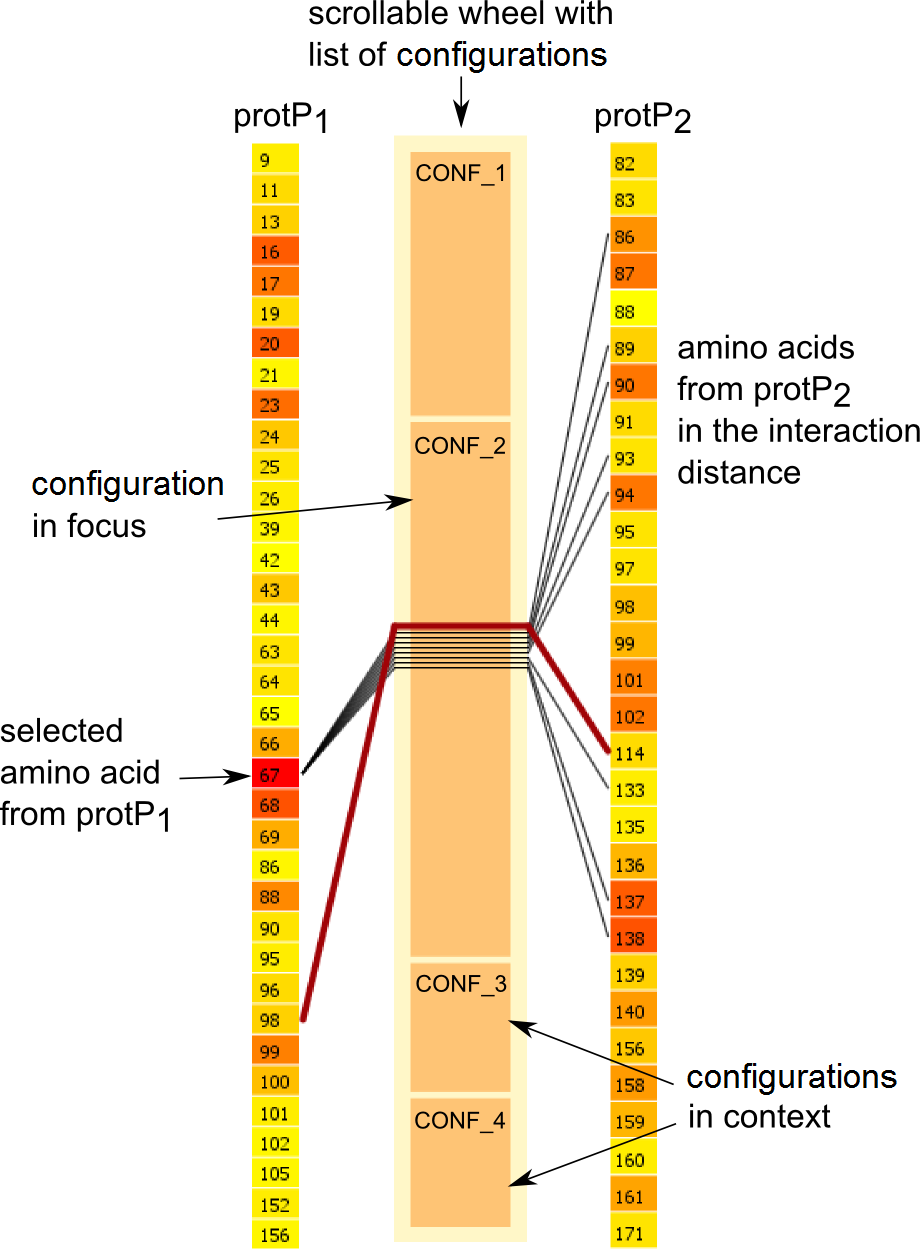
\includegraphics[width=0.8\columnwidth]{images/inco.png}
%  \caption{InCo lens view enables us to explore the interacting amino acids in the contact zone of a selected configuration.}
%  \label{fig:inco}
%\end{figure}

%The input configurations are coming from the filtering stage performed using the \MatView.
%he task is to iteratively search through this list of configurations.

%The currently investigated configuration in the middle contains the identifier of the configuration.

%The InCo lens view is further equipped with two lists of amino acids positioned on the left and right side of the central part.
%These lists are the same as in the case of the \MatView, i.e., they contain all amino acids present at least in one contact zone from $S$.
%The amino acids are again colored according to the frequency of their occurrence in $S$.



%The InCo lens view is highly interactive and closely linked with the \MatView.

%By combining the \MatView and InCo lens view, the domain expert can inspect the large input set of configurations and filter out those not satisfying the conditions derived from the preliminary knowledge about the interacting proteins.

%%%%%%%%%%%%%%%%%%%%%%%%%%%%%%%%%%%%%%%%%%%%%%%%%%%%%%%%%%%%

\subsection*{Exploded View}
The proteomics experts are already familiar with the manipulation of molecules in the three-dimensional (3D) environment, thus 3D representation has to be an integral part of the workflow.
Moreover, the 3D space helps to find answers for questions Q3-Q5, which are related to the appearance of the contact zones of selected configurations and the properties of interacting amino acids (expressed by different coloring schemes).
Exploring and comparing many structures in 3D at once suffer from problems like high overlaps, occlusion, and visual clutter (Figure~\ref{fig:case12}b). 
Traditionally used spatial representations are not sufficient.
To overcome these limitations, we adapt the exploded-view technique, in order to enlarge the distance between the interacting proteins. 
Figure~\ref{fig:case12}c shows the comparison of three configurations using our proposed \ExpView.

%To describe the principle of this technique in detail we need to introduce the following notation.
%Lets assume that a configuration $CONF_i(C(P_1,P_2))$ contains a contact zone $CZ(P_1,P_2)$ of the complex $C(P_1,P_2)$.
%This contact zone consists of two subsets of amino acids, each coming from one of the interacting proteins.
%Lets denote as $CZ(P_1)$ and $CZ(P_2)$ the part of the contact zone belonging to protein $P_1$ and $P_2$, respectively.
%One of the proteins $P_1$ or $P_2$ is marked as the \textbf{reference protein} $P_{ref}$.
%This can be done automatically by setting the protein read-in first as the reference one.
%Alternatively the user can select which of the loaded proteins should be the reference one.
%The set of reference proteins is then marked as $S(P_{ref})$.
%The second protein from $C(P_1,P_2)$ is automatically marked as the \textbf{paired protein} $P_{pair}$ and the set of these proteins is marked as $S(P_{pair})$.

%\begin{figure}[bt]
%  \centering
%  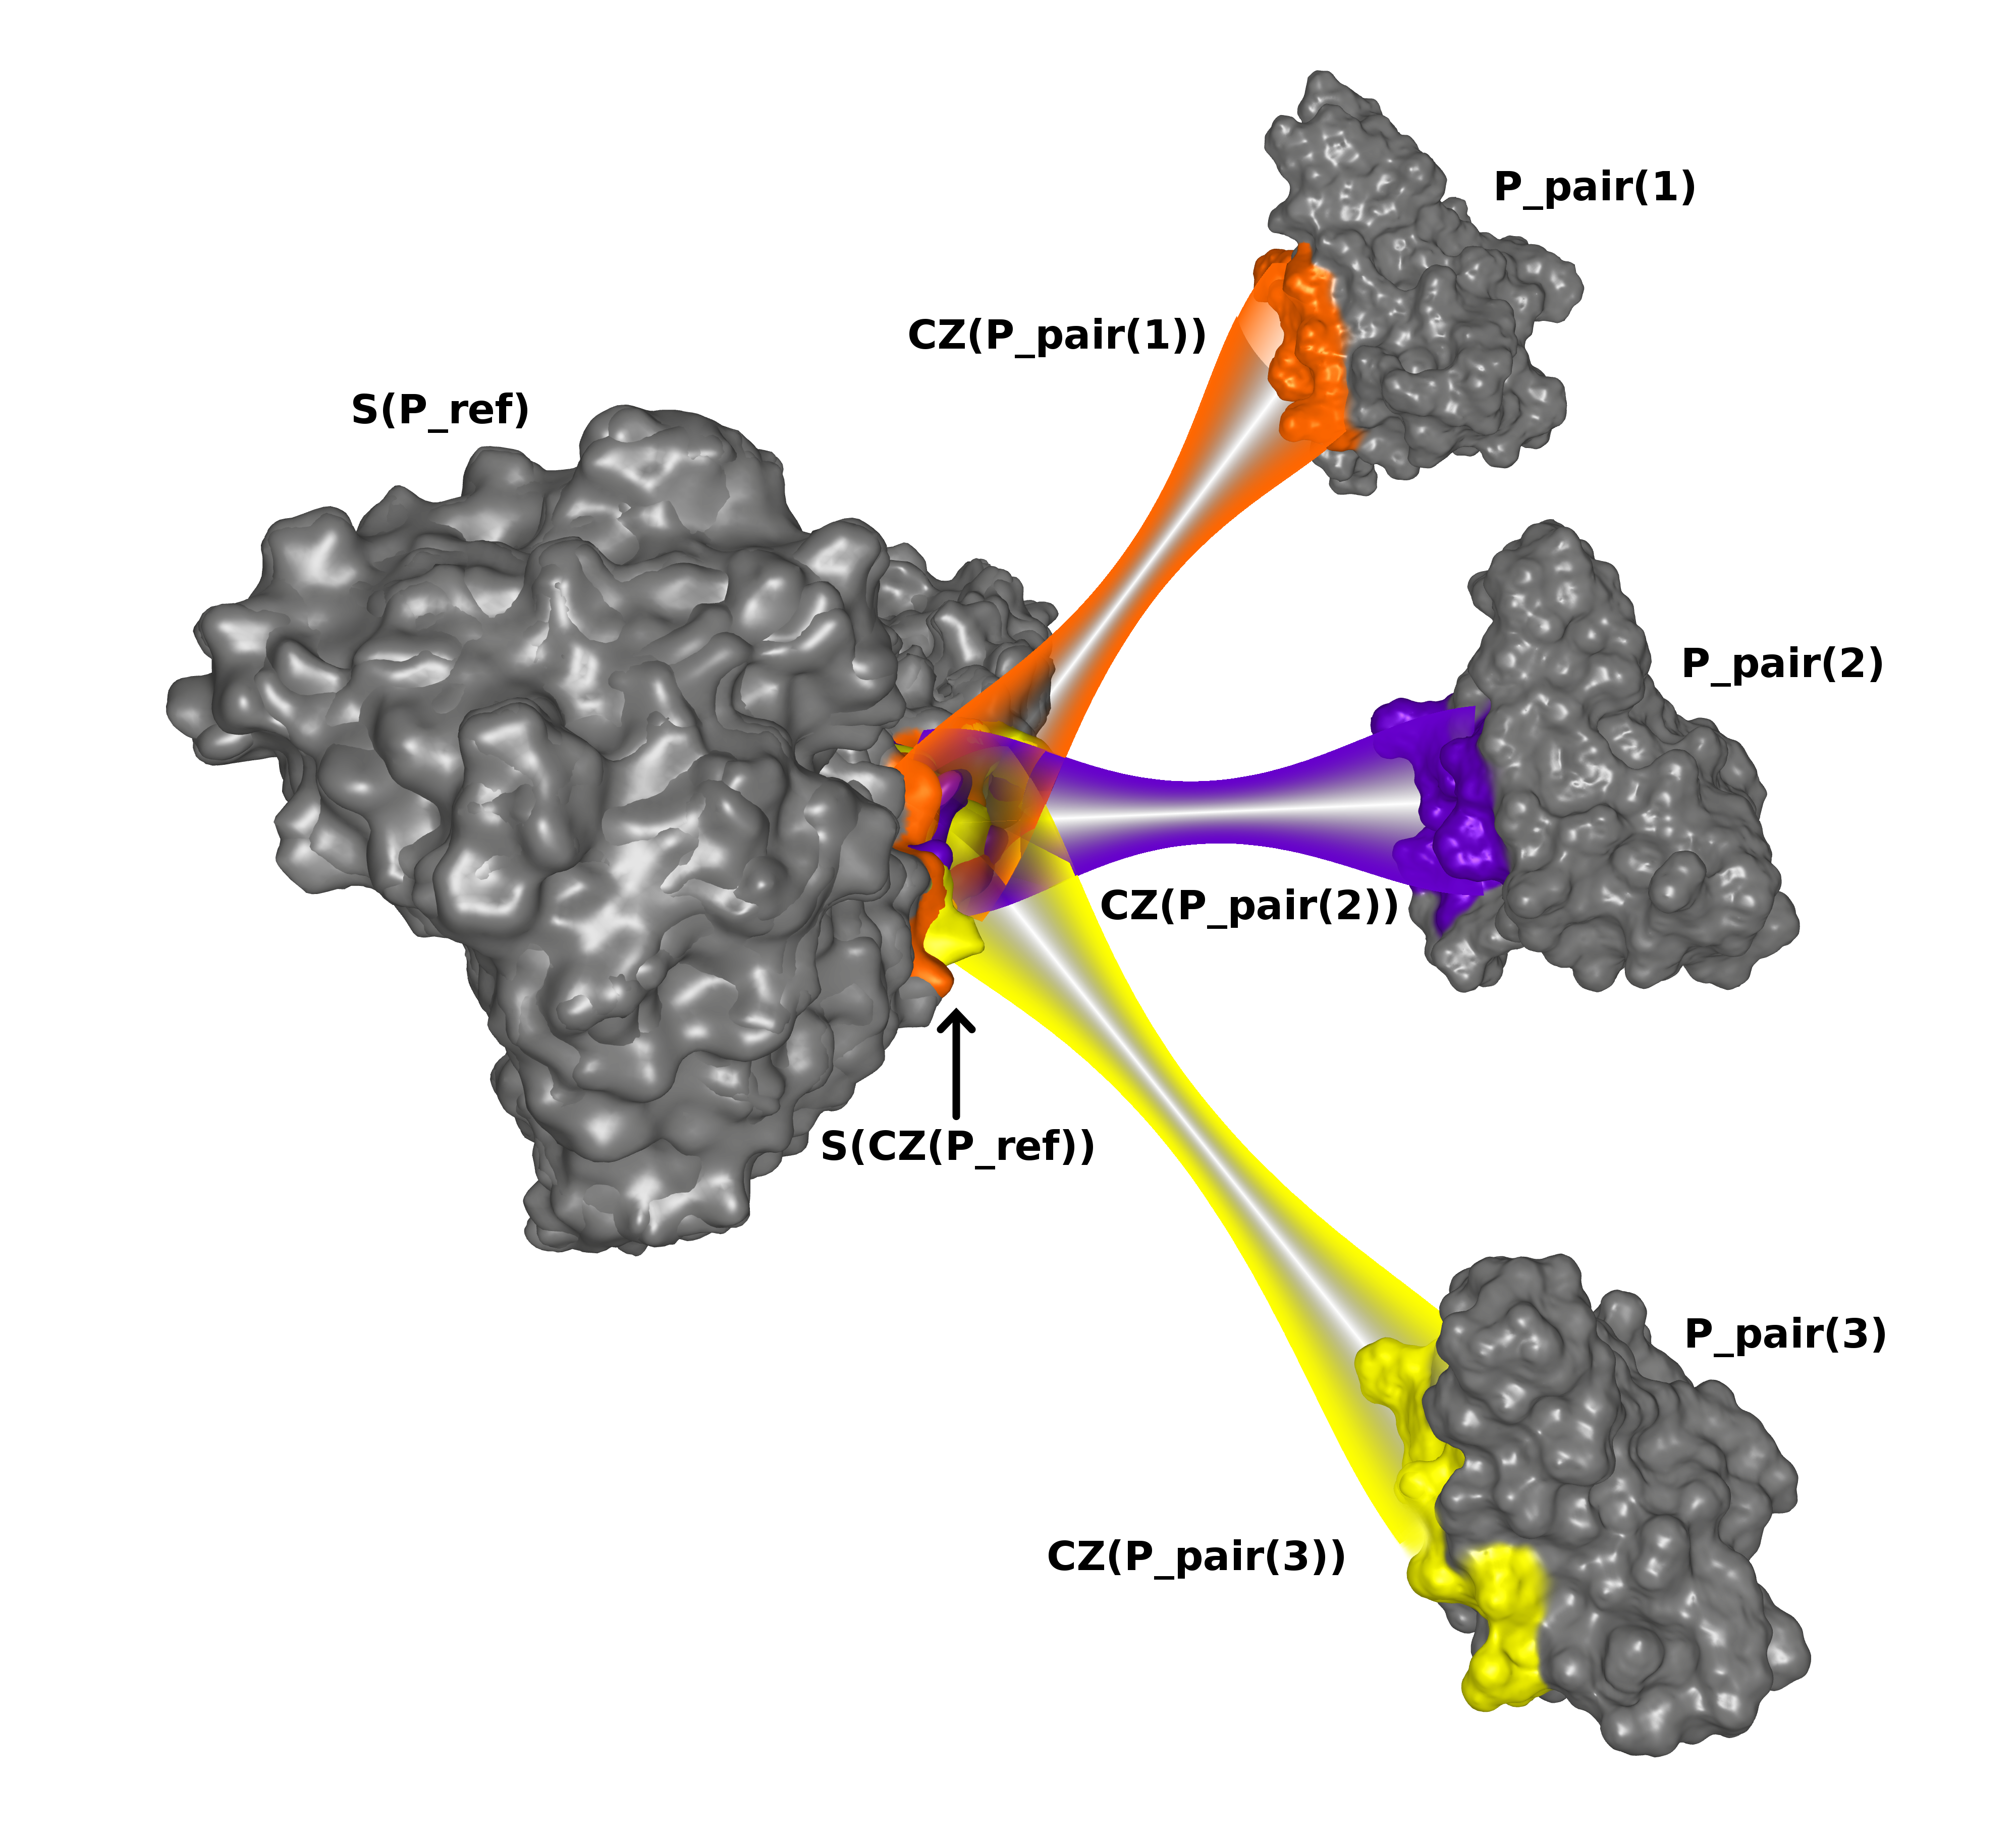
\includegraphics[width=1.0\columnwidth]{images/exploded.png}
%  \caption{\ExpView showing the interaction between three different configurations of the aligned reference protein (the biggest one) and its paired proteins (located nearby). Proteins are represented by their surfaces and the contact zones are colored.}
%  \label{fig:exploded}
%\end{figure}

The main principle of the \ExpView is the following.
First, all the reference proteins taken from the configurations selected by the \MatView are aligned using the Combinatorial Extensions of the structural-alignment algorithm~\cite{Shindyalov1998} so that their 3D spatial representations overlap (Figure~\ref{fig:case12}). 
Here, it is important to understand that the reference protein shown in Figure~\ref{fig:case12}b (the brown one) actually represents three overlapping aligned reference proteins, each coming from one configuration.
The set of paired proteins interacting with the reference proteins is positioned around the aligned reference proteins with the enlarged distance.

%As it is expected that the set of configurations selected in the previous stage contains more than one configuration, the proteins from $S(P_{pair})$ are overlapping significantly.
%Therefore, by increasing the distance between the proteins from $S(P_{ref})$ and $S(P_{pair})$ using exploded views can remedy this issue.

To ensure that the paired proteins in the Exploded view will not collide with each other, we employ a simple iterative force-directed placement algorithm, where the paired proteins repulse each other \cite{fruchterman1991graph}.
%For each pair of interacting proteins, the vector between $CZ(P_{ref})$ and $CZ(P_{pair})$ is computed. 
%$P_{pair}$ is then shifted along this vector away from $P_{ref}$ by a user-defined value. 
%This can lead to mutual collisions between the shifted $P_{pair}$ proteins.
%Thus, a relocation of the $P_{pair}$ proteins has to be applied to avoid these collisions. 
%We apply a heuristic but effective approach by putting all $P_{pair}$ proteins into a queue.
%For each $P_{pair}$ we detect collisions with all proteins remaining in the queue.
%The collision detection computation is based on the spherical bounding boxes of the proteins.
%If a collision is detected, we compute the $shift_{unproc}$ (unprocessed) vector for $P_{pair}$ as an averaged sum of vectors between $P_{pair}$ and all colliding proteins.
%Then we compute the $shift_{proc}$ (processed) vector for $P_{pair}$ shifted by the $shift_{unproc}$ vector in the same way for collisions with already processed proteins (which are not in the queue).
%The two shift vectors are then averaged and give the final $shift$ vector for $P_{pair}$, which is moved to its new non-colliding position.
%To avoid deadlocks, the whole relocation process is repeated until no collisions are detected anymore.
%The maximal number of repetitions corresponds to the number of $P_{pair}$ proteins (i.e., the number of processed configurations).
For each reference protein and its paired protein, the \ExpView keeps the information about their interaction.
If several configurations are exploded at once, the \ExpView contains many paired proteins arranged around the aligned reference proteins.
As the change in the position of the exploded proteins can cause disorientation in the scene, the pairing information between the corresponding reference proteins (aligned) and paired proteins ("exploded") is initially indicated as a partially transparent tube, that connects the centers of their contact zones.
The radius of the tube is modulated -- it is smaller in the middle of the tube to reduce the visual clutter.
Once the user gains the overview of the spatial arrangement of the proteins, the tube can be switched off.
The pairing information is also encoded by color -- for each configuration a different color is used.
If the contact zones contain the colliding amino acids (i.e., their mutual distance is less than 3~\AA), the residues are indicated by red color.

Figure~\ref{fig:case12} depicts a set of three configurations before (a, b) and after (c) applying the \ExpView.
The Exploded view removes the problem of overlapping paired proteins.
It also helps to see the shape and position of the contact zones.
However, this solution does not solve the problem that the contact zones still face each other so the user has to adjust the camera to observe the contact zones of the reference and paired proteins from a perpendicular viewing direction. 
Such a manipulation does not enable to see both contact zones simultaneously.
This problem is solved by the proposed \OpBook, presented in the following section.


%%%%%%%%%%%%%%%%%%%%%%%%%%%%%%%%%%%%%%%%%%%%%%%%%%%%%%%%%%%%

\subsection*{Open-Book View}
The \ExpView does not allow to observe both parts of a given contact zone simultaneously.
The proposed \OpBook is designed specifically to answer questions similar to Q5, which deals with a detailed exploration of one selected contact zone of the complex $C(P_1,P_2)$.
This involves the presentation of the information about different properties of individual amino acids forming the contact zone and their pairing.

The \OpBook is activated if the user selects one of the configurations from the \ExpView. 
The selection is performed by clicking on the connection tube of the desired configuration $CONF_i(C(P_1,P_2))$ in the \ExpView.
The other configurations are automatically hidden, the selected configuration returns to its initial position (before applying the \ExpView), and an animated transition of the opening of the $CONF_i(C(P_1,P_2))$ is launched.
When animating the opening, the reference and paired proteins are rotated and translated so that they are positioned next to each other and the contact zones are facing towards the observer (see Figure~\ref{fig:book}). 

The algorithm performing the opening computes the vectors defining the orientation of the contact zones (their normal vectors). 
From the normal vectors and the camera position, we compute the rotation angle, which is then applied to the reference and the paired protein.
%works as follows (illustrated in Figure~\ref{fig:bookSchema}).
%First we compute the center of mass of proteins $P_{ref}$ and $P_{pair}$, lets denote them by ${CM_P}_{ref}$ and ${CM_P}_{pair}$.
%Then we find also the center of mass of both $CZ(P_{ref})$ and $CZ(P_{pair})$, lets denote them ${CM}_{CZ(P_{ref})}$ and ${CM}_{CZ(P_{pair})}$.
%The vector between ${CM}_{CZ(P_{ref})}$ and ${CM}_{CZ(P_{pair})}$ in fact corresponds to the centerline of the tube connecting $P_{ref}$ and $P_{pair}$ in the \ExpView.
%Then we compute the vectors defining the orientation of the contact zones (normal vectors) for both $CZ(P_{ref})$ and $CZ(P_{pair})$ as $N_{P_{ref}} = %{CM}_{CZ(P_{pair})} - {CM}_{CZ(P_{ref})}$ and $N_{P_{pair}} = {CM}_{CZ(P_{ref})} - {CM}_{CZ(P_{pair})}$.
%In the following step the vectors heading from ${CM}_{P_{ref}}$ and ${CM}_{P_{pair}}$ to the camera position $CAM$ have to be computed.
%We will get them as $CAM_{P_{ref}} = CAM - {CM_P}_{ref}$ and $CAM_{P_{pair}} = CAM - {CM_P}_{pair}$.
%The normal and the camera vectors ($CAM_{P_{ref}}$, $CAM_{P_{pair}}$) are then used for the computation of the rotation angle which is then applied to $P_{ref}$ and $P_{pair}$.
%Furthermore, for each protein, it is necessary to find the appropriate rotation axis.
%This axis is anchored in the center of mass of the protein.
%It is perpendicular to the normal and camera vectors and is computed as their cross product $cross(N_{P_{ref}},CAM_{P_{ref}})$, $cross(N_{P_{pair}},CAM_{P_{pair}})$ %respectively.%
%Then the $P_{ref}$ and $P_{pair}$ proteins are rotated around the computed rotation axes with the determined rotation angles.
To maintain the information about the pairing of amino acids, the user can visualize also individual connections between these pairs by simple lines.

%\begin{figure}[bt]
%  \centering
%  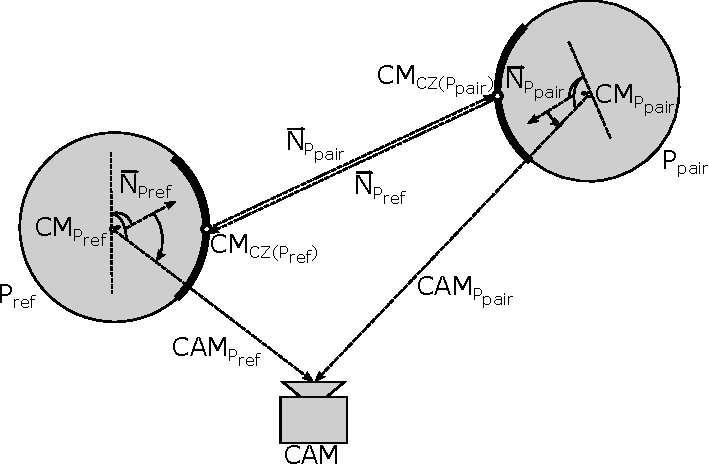
\includegraphics[width=1.0\columnwidth]{images/openBook2.pdf}
%  \caption{Illustration of the Open-Book algorithm.}
%  \label{fig:bookSchema}
%\end{figure}

The contact zones represented by their surfaces can be color-coded according to multiple criteria.
The color can encode the distance between the amino acids or it represents different physico-chemical properties of the amino acids or their atoms, such as hydrophobicity or partial charges.
The coloring scheme used in the \MatView represents so called conservation of the amino acids in all configurations.
It can be used for coloring the contact zone as well.
The surfaces can be augmented with labels to inform the users about the type and the identifier of individual amino acids.

In both, the \ExpView and the \OpBook, a protein can be represented also by other traditionally used visualization styles, such as cartoon, spheres, balls\&sticks, sticks, etc.
Moreover, these methods can be combined. 
For example, the proteins can be represented by the cartoon style and the amino acids in the contact zones can be visualized using the sticks representation to see their spatial orientation.% (see Figure~\ref{fig:contact}).

%The combination of the \ExpView and the \OpBook is useful for the exploration of individual pairs.
If the task is to compare individual configurations with respect to the pairs of the interacting amino acids, a further drill-down is necessary.
Therefore, in the next section, we propose another abstracted view supporting mainly the comparison of the paired amino acids in individual contact zones of selected configurations.

%%%%%%%%%%%%%%%%%%%%%%%%%%%%%%%%%%%%%%%%%%%%%%%%%%%%%%%%%%%%

\subsection*{Contact-Zone List-View}
The \CoZoListView helps to answer questions related to the comparison of the contact zones on the level of individual amino acids, such as in Q6.
The list for one configuration consists of two sets of amino acids in the contact zones, each set coming from one interacting protein (see Figure~\ref{fig:list}).
The left part of the view contains all amino acids coming by default from the reference protein, the right part is formed by their interaction counterparts in the paired protein.
However, the order of proteins in the list-view can be changed.
The order depends on the current task, i.e., if we want to compare the constitution of contact zones of the reference or the paired protein in the given configurations.
The view contains all possible connections (w.r.t. the distance) between the amino acids from both contact zones.
To avoid intersections of lines representing the connections, some amino acids on the right side are repeated -- one instance for each reference protein amino acid within a user defined distance. 
This solution was adopted because without these repetitions there would be many line intersections, which substantially decreases the readability of the representation (see Figure~/ref{fig:pdbsum}b).

For each configuration, one list-view is created and all list-views are juxtapositioned so the user can see and visually compare the constitution of the contact zones of all selected configurations.
%The horizontal ordering of the views is user-defined.
The user can modify this representation by changing the color, which can encode different properties of the amino acids mapped onto their corresponding rectangles.
The properties are the same as those mapped onto the surface of the contact zone in the Exploded view and the Open-Book view.
The left part of the list can then be sorted according to these properties (see Figure~\ref{fig:sorting}).
Moreover, by clicking on individual rectangles representing the amino acids, the corresponding amino acids are selected in the 3D view as well.

The principle steps for building the \CoZoListView are the following.
For all configurations, which should be visualized in the \CoZoListView, we find the interacting pairs of amino acids in their contact zones.
%\textcolor{red}{...we find the closest interacting pair of amino acids.
%It is the same pair as the one represented by the default polyline in the InCo view. -- there is still possibility to show just the closest, but now we take all detected contacts by default, as JP requested}
Then, the list of amino acids present in all reference proteins of the selected configurations is created.
Now, for each configuration, we take the interacting amino acids from the paired proteins, sort them according to a selected criterion (e.g., hydrophobicity), and add them to the \CoZoListView.
The amino acids in the left part of the \CoZoListView are always sorted in the same way for all depicted configurations.
Similarly to the \MatView, the user can select a primary configuration to which all the remaining configurations are compared (see Figure~\ref{fig:list}b), using the proposed ranking score algorithm, described in Section Matrix View.
The \CoZoList plots the configurations ordered from left to right by the similarity score from the most similar to the least similar ones.
The \CoZoListView of the primary configuration is always displayed as the first one from the left side of the view.

The user can select between two visualization modes -- the \textit{compare} and the \textit{compact} list-view.
In the \textit{compare} mode, the amino acids from the contact zone of the primary configuration that are not present in the contact zone of any other configuration, are depicted as white rectangles with labels giving the names of the missing amino acids (see Figure~\ref{fig:list}b).
The \textit{compact} mode omits these missing amino acids to save space.
In both modes, the matches to amino acids in the primary configuration are highlighted with red bordered rectangles and connecting lines.
This way, the user can immediately see which amino acids are present in both, the primary configuration as well as the other configurations, and which amino acids are missing.
To guide the visual comparison, we also introduce interactive highlighting and, if necessary, zooming to corresponding amino acids in different configurations.

%TODO add info about the comparison with the reference configuration! Then it shows, what is missing or redundant in individual configurations.

%\section{User Interaction}
%Some of the interaction possibilities were already described along with the explanation of the individual proposed visualizations.
%All suggested visualizations are interactively linked to support the workflow of the biochemists as much as possible.
%This means that by the selection of cells in the \MatView the user automatically filters out those configurations which do not fulfill the filter criteria and these configurations are further omitted from the other views as well.
%Of course, the user can at anytime return to the beginning of the process. 
%By the iterative refinement of the filtering using the matrix and lens views the set of configurations can be further reduced.
%Another possible scenario is that the user finds out that some of the promising configurations were filtered out at the beginning.
%Such configurations can then be included back into the exploration process.

\section*{Results and discussion}
%All presented techniques and their integration into the proposed COZOID tool were designed in a tight collaboration between the domain experts from the field of visualization and the field of functional proteomics.
%The group consists of a senior proteomic expert, two junior researchers, and the testing was performed by eight students of proteomics.
%Our current main research focus in proteomics is on the structure maintenance of chromosome (SMC) complexes~\cite{Palecek2015}. 
%The SMC complexes are the key players in the chromatin organization where they ensure the stability and dynamics of chromosomes. 
%The researchers analyze the architecture and function of such complexes using a variety of experimental approaches. 
%The goal is to uncover the way the subunits of these complexes interact with each other and execute unique functions of these complexes~\cite{Gligoris}. 
%A visual representation of such an information is highly beneficial because it helps to reveal the spatial relationships between the subunits in an intuitive way.

To demonstrate the usability of our proposed techniques, we selected representatives of three basic types of PPI patterns,  present in the SMC complexes~\cite{Palecek2015}. 
The SMC (Structure Maintenance of Chromosome) complexes are the key players in the chromatin organization where they ensure the stability and dynamics of chromosomes. The way the subunits of these complexes interact with each other is key for their functions~\cite{Gligoris}.
A visual representation of such an information is highly benecial as it helps to reveal the spatial relationships between the subunits in an intuitive way.
%These patterns differ in the shape of the contact zones and interacting protein domains.
The three basic PPI types are the coiled-coil interaction, the pocket-string interaction, and the surface-surface interaction~\cite{alberts02molecular}.
In the following subsections, we demonstrate the usefulness of our proposed visualizations on these three types of interaction.

\subsection*{Surface-Surface Interaction}
The most frequent surface-surface interaction type was tested on NSE1 and NSE3 proteins of SMC5/6 complex. 
This interaction has been analyzed as it represents the dimer of kite proteins, which are critical for the function of the eukaryotic SMC5/6 and the bacterial SMC complexes~\cite{Zabrady2016,Palecek2015,Doyle2010}. 

The crystal structure of the human NSE1-NSE3 dimer was already examined in detail and the resulting configuration is already published in the PDBsum database under the PDB identifier 3NW0. 
Therefore, it can serve us as a testing primary complex for both computational tools as well as for our proposed visualizations.
%The senior proteomic expert conducting this study provided us with the docking results and his prior knowledge about the \textcolor{red}{initial pair of interacting amino acids}.
To restrict the set of possible docking configurations, we selected the web version of the HADDOCK tool and a pair of interacting amino acids, i.e., methionine with ID 23 from the reference protein and leucine with ID 97 from the paired protein (Figure~\ref{fig:pdbsum}b).
This selection was based on the experimental data from the previous works~\cite{Doyle2010,Hudson2011,Kozakova,Crabben}.
The HADDOCK analysis resulted in 40 possible configurations.
HADDOCK groups the configurations into clusters, according to their similarity, which is defined internally by the HADDOCK score.
In our case, it led to 10 clusters, each containing 4 configurations.

All computed configurations were loaded into our COZOID visualization system, which interactively links all proposed visualizations.
From these configurations, first the \MatView was computed, which contains the frequencies of all pairs of amino acids within the interaction distance within these 40 configurations.
The matrix identified configurations containing the pairs of interacting amino acids with the interaction distances smaller than 4 \AA.
In our particular case, the leucine 97 and methionine 23 amino acids were in the contact distance in only three configurations out of the initial 40 (Figure~\ref{fig:matrixlens}). 
The Matrix view helped to filter these immediately by simple interaction with the view. 
The remaining 37 configurations were automatically hidden in the remaining views.
%Of course, the configurations not fulfilling this criterion could be automatically discarded and even not integrated into the \MatView.
%But this is not desirable because the contact zones are formed by many interacting amino acids and the matrix showing their frequency gives the user the information that even when the selected pair is not in the interaction distance the configuration can  still be promising because of the other interacting pairs.
%Moreover, the algorithm for the computation of amino acid pairs takes strictly the threshold of 5 \AA.
%So if the distance is only slightly bigger, the pair is not detected.

%The configurations preselected by the \MatView can be further scrutinized using the InCo lens view.
%This can potentially reduce the set of configurations passed to the next stage where the configurations are explored in three-dimensional space. 
%In our case study the InCo lens view helped the proteomic expert to confirm the correctness of the initial selection made through the \MatView.
%For all five configurations, it confirmed that the most frequent amino acids are in the interaction distance.
%Thus there is a high probability that these will also occur in the contact zone of the resulting biochemically relevant configuration.

In the next step, we switched to the \CoZoListView and compared the list of amino acids of the 3NW0 crystal structure with the lists of all three selected configurations.
Figure~\ref{fig:case3} shows the comparison between the 3NW0 structure and three selected HADDOCK configurations.
%The left part of all views contains the list of amino acids in the contact zone of $P_{ref}$, the right part represents $P_{pair}$.

Even from the given part of the \CoZoListView, the similarities and differences between the crystal 3NW0 (in the leftmost list) and the three selected HADDOCK configurations on the level of individual amino acids are clearly visible.
In addition, the pairs of the interacting amino acids identical to the 3NW0 crystal structure are highlighted (red lines in Figure~\ref{fig:case3}). 
The left-to-right order of the modeled configurations in Figure~\ref{fig:case3} reflects their similarity to the primary crystal structure, based on the number of identical pairs of amino acids (the best model is next to the crystal).

%From this view it is clearly visible that the contact zone of the configuration $CONF_5(C(P_{ref},P_{pair}))$ contains significantly fewer amino acids in $P_{ref}$ than the other configurations. 
%The amino acids which are missing in this configuration but are present in the others are also detected very easily.
%On the other hand, configurations $CONF_1(C(P_{ref},P_{pair}))$, and $CONF_3(C(P_{ref},P_{pair}))$ are the most similar with respect to the number and type of amino acids. 
%The configurations can be compared also pairwise and the \CoZoListView reveals the differences in their sets of amino acids.

%At the end of this process the domain expert confirmed that he obtained enough relevant information to decide that the configuration $CONF_5(C(P_{ref},P_{pair}))$ is not the relevant one and the remaining, very similar, configurations are worthwhile to test in the laboratory.
%He gained enough information to select possible candidate amino acids for mutation which should lead to the strengthening of the interaction within this complex.

%Finally the domain expert confirmed the correctness of the selection by the comparison of the resulting configurations with the \textcolor{blue}{3NW0} structure from the PDBsum database.
%He confirmed that the conducted case study demonstrated the usefulness of our proposed methods namely in two cases.
%The first case helps to evaluate the correctness of the outputs of the existing computational tools when testing them on an already known protein complex (as in our case).
%By comparing the known information about the complex with the outputs of the tool the user has an idea about the relevance of the results.
%In our case study we came to the conclusion that the HADDOCK results were relevant only in 10\% of all resulting configurations.
%The same test was performed for the PyDock tool~\cite{pydock} and the percentage of the relevant results was even lower.
%However, the conclusion about the correctness of the computational tools can be made only after performing a much larger set of testing.

Finally, the 3NW0 crystal and three selected configurations were explored using the 3D representations with the aim to explore the constitution, the mutual distances, and the properties of the contact zones in detail.
In 3NW0, the first NSE1 interacting protein was selected as the reference protein and all three configurations were aligned with respect to the paired proteins.
The paired proteins were positioned around the reference one.
Figure~\ref{fig:case12}a shows the situation where the three selected configurations are visualized using the commonly available method.
The configurations are represented as surfaces and the contact zones are highlighted using different colors.
However, the most interesting parts, i.e., the contact zones, are hidden (Figure~\ref{fig:case12}b).

Our \ExpView overcomes this limitation so the individual contact zones of all paired proteins are clearly visible (Figure~\ref{fig:case12}c).
Moreover, if we point the camera towards the aligned reference proteins, the differences between the positions of the contact zones in the reference proteins can be observed as well.
%If rotating the scene, the user can easily lose the information about the direction of the shift between the proteins.
The \ExpView representation gave us the information about the mutual positioning of the individual configurations with respect to the positions of the contact zones.

Using our tool, the investigation can go even deeper into the level where individual contact zones can be explored in detail using the \OpBook.
By animating the opening of the protein complex, we were able to look inside the contact zone.
The enhancements of the \OpBook, i.e., labeling the surface of the contact zones with the names of the corresponding amino acids, and coloring them according to different properties, were highly beneficial for the exploration of the physico-chemical and geometric properties of the individual amino acids.% appreciated by the domain expert.



%This helped to clearly understand the constitution of the contact zone and all its properties.
%After the exploration using the OB view the expert returned to the unopened view and used the possibility to visualize the polypeptidic chains of the interacting proteins in a more abstracted way employing the cartoon representation. 
%This allowed him to add the detailed representation of interesting pairs of amino acids selected using the OB view.
%These pairs were subsequently visualized using the balls\&sticks method so the mutual orientation of the amino acids was visible.
%%(see Figure~\ref{fig:contact}).

%%\begin{figure}[bt]
%%  \centering
%%  \includegraphics[width=0.8\columnwidth]{contact.png}
%%  \caption{Cartoon representation of the interacting proteins where green color corresponds to the contact zone. Leucine 97 and Methionine 23 interacting amino acids are highlighted using the balls\&sticks method and the color corresponds to their hydrophobicity. \textcolor{red}{TODO change image}}
%%  \label{fig:contact}
%%\end{figure}


%The second possible case where our visualizations can be highly beneficial is related to the research of newly modeled protein complexes.
%The researchers are often taking the known crystal structure of a complex and are modeling its homologous structures in order to create a variant of the known complex for another organism.
%These new homologous structures are very similar to the reference crystal structure but even slight differences can influence the interaction between the proteins substantially.
%Therefore, the detailed exploration of these differences is crucial and here our proposed visualizations can play an important role as well.

\subsection*{Coiled-Coil Interaction}
For the second type of interaction, we picked the SMC3 coiled-coil arm of the SMC complex~\cite{Gligoris}.
The interaction site is formed by two helical fragments of the SMC3 protein.
The primary structure is published under the PDB identifier 4UX3~\cite{pmid25414305}.  

Using this structure, the results of both the HADDOCK and the PyDock tools were tested.
The HADDOCK results contained 40 output configurations.
Using the \MatView, we set the interaction distance threshold between 3 and 5~\AA~and selected the methionine 186 and isoleucine 1030 as the initial pair of interacting amino acids (Figure~\ref{fig:coiled_haddock_mat}). 
These amino acids were used as the input restraints for the HADDOCK computation as well.
These restraints were applied to select correct configurations in the \MatView (Figure~\ref{fig:coiled_haddock_mat}).

Next, the selected configurations were structurally aligned in the 3D space to the primary 4UX3 structure.
Afterwards, we selected the first amino acid (A172) within the respective helices and visually compared their positions in the 3D view.
In this case, it was not even necessary to use other views to see that the preselected HADDOCK configurations exhibited a wrong orientation of the aligned helices. 
In all output models, these A172 amino acids were located on the opposite side in comparison with the primary crystal 4UX3 (see Figure~\ref{fig:coiled_haddock}). 
The 3D view of COZOID helped to reveal this misorientation intuitively and quickly, without a detailed exploration of all HADDOCK configurations one by one.

As for the PyDock results, 28 out of 100 output PyDock models were selected using the \MatView with the interaction pair M186 and I1030 used to filter the results.
The next visual selection (based on A172 position judgment) provided us with 14 models with correct orientation (see Figure~\ref{fig:selection2SMC3PyDock}).

In the final step, we compared the \CoZoLists of the selected models with the original crystal structure (4UX3). 
Figure~\ref{fig:coiled2} shows the similarities (highlighted in red) of one of the selected models to the crystal. It is the best model, which fits the crystal structure very well. The \ExpView comparison of the contact zone of the crystal structure and the selected model can be seen in Figure~\ref{fig:selection_4_final_SMC3_PyDock}.

\subsection*{Pocket-String Interaction}
For the pocket-string interaction type, we selected the interaction present in the crystal structure of the MukE-MukF complex --  the PDB identifier 3EUH~\cite{Woo}. 
The pocket is formed by the winged helix domain of the MukE protein, while one of the MukF helical fragments is sitting inside the MukE pocket (Figure~\ref{fig:MukEF_crystal_3EUH_selected}a). 
This time, we selected the valine 200 and arginine 300 as the pair of amino acids for the docking restraint. 
These were the closest contact amino acids of the structure, as can be seen from the \CoZoList ordered by the distance of the interacting amino acids (see Figure~\ref{fig:list_pocket_string}), as well as from the \OpBook of the crystal structure (Figure~\ref{fig:MukEF_crystal_3EUH_selected}b). 

The docking models were again generated with both HADDOCK and PyDock docking tools.
The HADDOCK run resulted in 32 output configurations, which were first scrutinized using the \MatView, using the initial V200-R300 amino acid pair. 
This first selection step filtered away only 8 models, leaving 24 models for further analysis. 
Then, we repeated the \MatView filtering using the second tightest amino acid contact in the crystal -- the tyrosine 110 and arginine 302 (Figure~\ref{fig:MukEF_crystal_3EUH_selected}b). 
This filtration resulted in 6 docking models. 
The \CoZoLists of these models were compared with the original crystal structure (3EUH), resulting in an ordered list of the best models (Figure~\ref{fig:list_pocket_string}).
The visual exploration confirmed that the first model from the \CoZoList fits best to the original structure (Figure~\ref{fig:MukEF_selection_3_best_pair}). 

The PyDock docking provided 100 models, which were analyzed in the same way as the HADDOCK models. 
The selection steps with the \MatView resulted in 32 and then 19 models, respectively. 
The \CoZoLists of these models were then compared with the original crystal structure.
The models matching most closely to the original crystal structure, detected using the \CoZoList, were then visually explored in 3D using the \ExpView and the \OpBook.
This step revealed that the best five models from the list are very close to the original crystal, but none of them fits precisely to the crystal structure.

Here, we took the advantage of our test set-up (using the tightest contacts between the interacting amino acids) and altered the interaction distance parameter in the \MatView for the selection procedure. 
All PyDOCK models were reevaluated with the distance parameter 4 \AA~(compared to the previous 5 \AA~default parameter). 
As expected, fewer configurations containing the V200-R300 and Y110-R302 amino acid pairs within 4 \AA~distance were found -- the \MatView selection steps resulted in 21 and 13 models, respectively.
However, the altered distance parameter also resulted in different ranking of the configurations in \CoZoLists.
Figure~\ref{fig:list_3euh} shows the comparison of \CoZoLists of 3EUH crystal structures computed with 5 \AA~and 4 \AA~distance parameter respectively.
It can be seen, that the decreased distance parameter eliminated several amino acid pairs with distance higher than 4~\AA~from the \CoZoList of the crystal structure.
The eliminated pairs were not considered in the new \CoZoList ranking, where five models most similar to the crystal were again selected (Figure~\ref{fig:pydock_pocket_string}a). 
%Based on the \CoZoLists and the 3D view analysis using the \ExpView and the \OpBook, 
Four of these five models overlapped with the five best models detected with the previous system set-up, however, a new model with closer match was identified (Figure~\ref{fig:pydock_pocket_string}b).

This test indicates the robustness of our tool at different parameter settings and its potential for the proteomic experimental use.
Our tool can be used also for selecting an alternative input pair of interacting amino acids, which then serves as the input for the computational tools.
These amino acids might be selected based on the COZOID analysis of the 3NW0 crystal -- using the \MatView or the \ExpView (searching for the most central and the closest amino acids).

Altogether, COZOID helped us to quickly select the best docking configuration using several visualization approaches. 
First, the \MatView allowed us to pick models containing a particular pair of interacting amino acids. 
Next, with the \CoZoList, we sorted these models based on the similarity of their contact zones with the original crystal structure. 
Using the 3D \ExpView, the best model was determined and confirmed. 
While the Exploded view is already available in some of the current 3D visualization tools, the power of its combination with our other proposed approaches lies in the speed, user-friendly design, and high interactivity of the selection mechanism. 
In addition, a similar workflow can be applied to the selection of the docking models of homologous proteins, not available in the PDB database, yet very often used when different model organisms are employed in the proteomic studies.
 
For example, our \CoZoList can be used in the experimental design of mutants by replacing the key contact residues. 
This tool can be used by the proteomic expert to select amino acids in the contact zones that could be mutated, i.e., replaced by other amino acids.
The ultimate goal of such a mutation can be to strengthen the interactions in the contact zone or, otherwise, completely destroy the interaction between the involved proteins. 


\section*{Conclusions}
In this paper, we have presented COZOID, a novel tool for the visual exploration of configurations of two interacting proteins. 
It introduces a set of visualization methods for the exploration and evaluation of the proteomic relevance of large sets of configurations, detected by the existing computational tools.
Our proposed methods were designed to follow and support the workflow of the proteomic experts.
We described the design rationale and the principles of these methods, as well as their linking and interaction possibilities. 
%The methods were tested by the proteomic experts on real datasets for SMC complexes and we demonstrated the usability on three studies, covering the most common interaction patterns.
%The domain experts confirmed that our proposed solution provides them with information, which was very hard or even impossible to get using the previously available methods.
%They confirmed that using our solution, their exploration process can lead to a satisfying conclusion about the biochemical relevance of individual configurations much faster.
We tested these methods on real datasets of the SMC complex subunits and we demonstrated their usability in three studies, covering the most common interaction types.
Our proposed solution provides the proteomic experts with information, which was very hard or even impossible to get using the previously available methods.
The studies confirmed that using our solution, the exploration process can lead to a satisfying conclusion about the proteomical relevance of individual configurations much faster.
The system enables iterative filtering of the configurations that do not satisfy given criteria in the individual stages of the workflow.

In the future, we plan to focus on the extension of our proposed techniques to cases where the user has no a priori knowledge about the protein complex, but can feed in experimental data from, e.g., mutagenesis or crosslink analysis.

%% if specified like this the section will be committed in review mode
%%%%%%%%%%%%%%%%%%%%%%%%%%%%%%%%%%%%%%%%%%%%%%
%%                                          %%
%% Backmatter begins here                   %%
%%                                          %%
%%%%%%%%%%%%%%%%%%%%%%%%%%%%%%%%%%%%%%%%%%%%%%

\begin{backmatter}
\section*{Availability of data and materials}
Data and materials are available upon request.

\section*{Competing interests}
  The authors declare that they have no competing interests.

\section*{Author's contributions}
K. Furmanov\'{a} participated on the design of the tool, its implementation, and paper editing.  J. By\v{s}ka contributed to the implementation. I. Viola and E. M. Gr\"{o}ller contributed to the design of visualizations and interactions of the tool. J. J. Pale\v{c}ek contributed to the design and was responsible for testing and evaluation of the tool and paper editing. B. Kozl\'{i}kov\'{a} contributed to the design, paper writing, and was coordinating the team and activities.

\section*{Acknowledgements}
This work was supported through grants from the Vienna Science and Technology Fund (WWTF) through project VRG11-010, the OeAD ICM and MSMT-1492/2015-1 through project CZ 17/2015, the PhysioIllustration research project 218023 funded by the Norwegian Research Council, the Ministry of Education, Youth and Sports of the Czech Republic project CEITEC 2020 (LQ1601), and an Internal Masaryk University grant (MU/0822/2015). We also acknowledge the members of Palecek lab for their participation in the COZOID testing. 

%%%%%%%%%%%%%%%%%%%%%%%%%%%%%%%%%%%%%%%%%%%%%%%%%%%%%%%%%%%%%
%%                  The Bibliography                       %%
%%                                                         %%
%%  Bmc_mathpys.bst  will be used to                       %%
%%  create a .BBL file for submission.                     %%
%%  After submission of the .TEX file,                     %%
%%  you will be prompted to submit your .BBL file.         %%
%%                                                         %%
%%                                                         %%
%%  Note that the displayed Bibliography will not          %%
%%  necessarily be rendered by Latex exactly as specified  %%
%%  in the online Instructions for Authors.                %%
%%                                                         %%
%%%%%%%%%%%%%%%%%%%%%%%%%%%%%%%%%%%%%%%%%%%%%%%%%%%%%%%%%%%%%

% if your bibliography is in bibtex format, use those commands:
\bibliographystyle{bmc-mathphys} % Style BST file (bmc-mathphys, vancouver, spbasic).
\bibliography{bmc_article}      % Bibliography file (usually '*.bib' )
% for author-year bibliography (bmc-mathphys or spbasic)
% a) write to bib file (bmc-mathphys only)
% @settings{label, options="nameyear"}
% b) uncomment next line
%\nocite{label}

% or include bibliography directly:
% \begin{thebibliography}
% \bibitem{b1}
% \end{thebibliography}

%%%%%%%%%%%%%%%%%%%%%%%%%%%%%%%%%%%
%%                               %%
%% Figures                       %%
%%                               %%
%% NB: this is for captions and  %%
%% Titles. All graphics must be  %%
%% submitted separately and NOT  %%
%% included in the Tex document  %%
%%                               %%
%%%%%%%%%%%%%%%%%%%%%%%%%%%%%%%%%%%

%%
%% Do not use \listoffigures as most will included as separate files

\section*{Figures}
  \begin{figure}[h!]
  \centering
  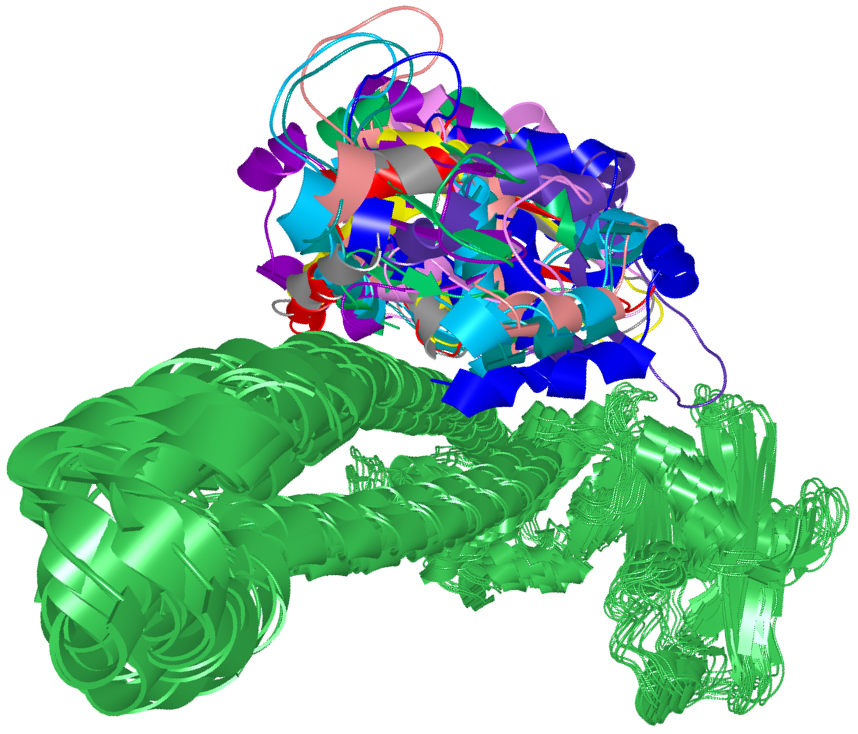
\includegraphics[width=0.9\columnwidth]{images/figure1.png}
 \caption{\csentence{Traditionally used 3D visual representation of configurations.}
	Typical visual representation of configurations used by the proteomic experts that suffers from substantial visual clutter. It superposes several possible configurations between two proteins and visualizes them using the cartoon model. The set of green protein instances corresponds to one of the interacting proteins, the colored components represent the second protein in different spatial configurations.}
  \label{fig:problem}
\end{figure}

\begin{figure}[h!]
  \centering	
  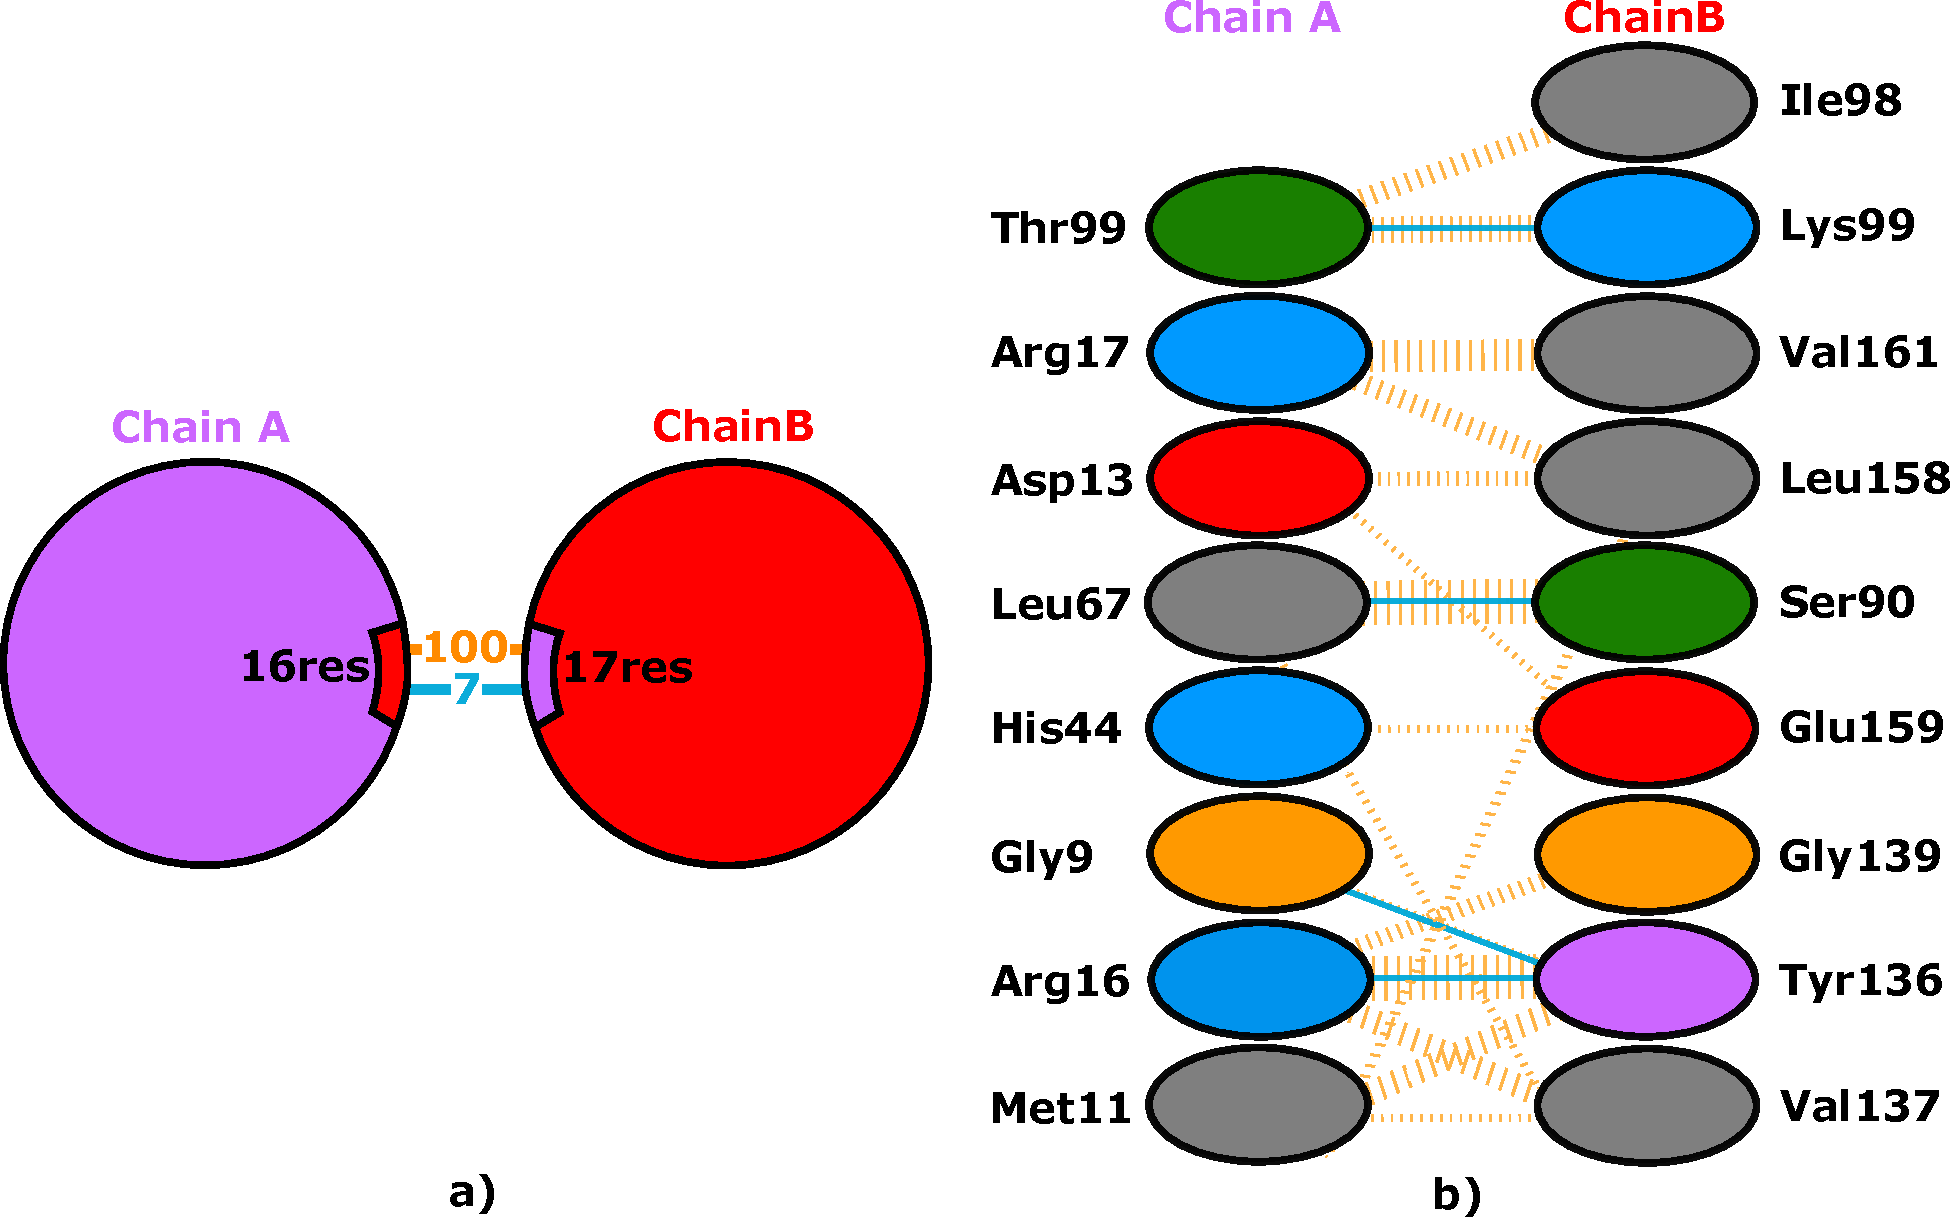
\includegraphics[width=0.9\columnwidth]{images/figure2.pdf}
  \caption{\csentence{NSE1-NSE3 complex representation in PDBsum.}
    Two abstracted visualizations of the NSE1-NSE3 complex with PDB ID 3NW0 available in the PDBsum database. (a) Overview representation showing the number of amino acids in the contact zones and the types of interactions. (b) Part of the list of interacting amino acids along with individual interactions and their strength. Images taken from the PDBsum database~\cite{pdbsum}.}
    \label{fig:pdbsum}
\end{figure}

\begin{figure}[h!]
  \centering	
  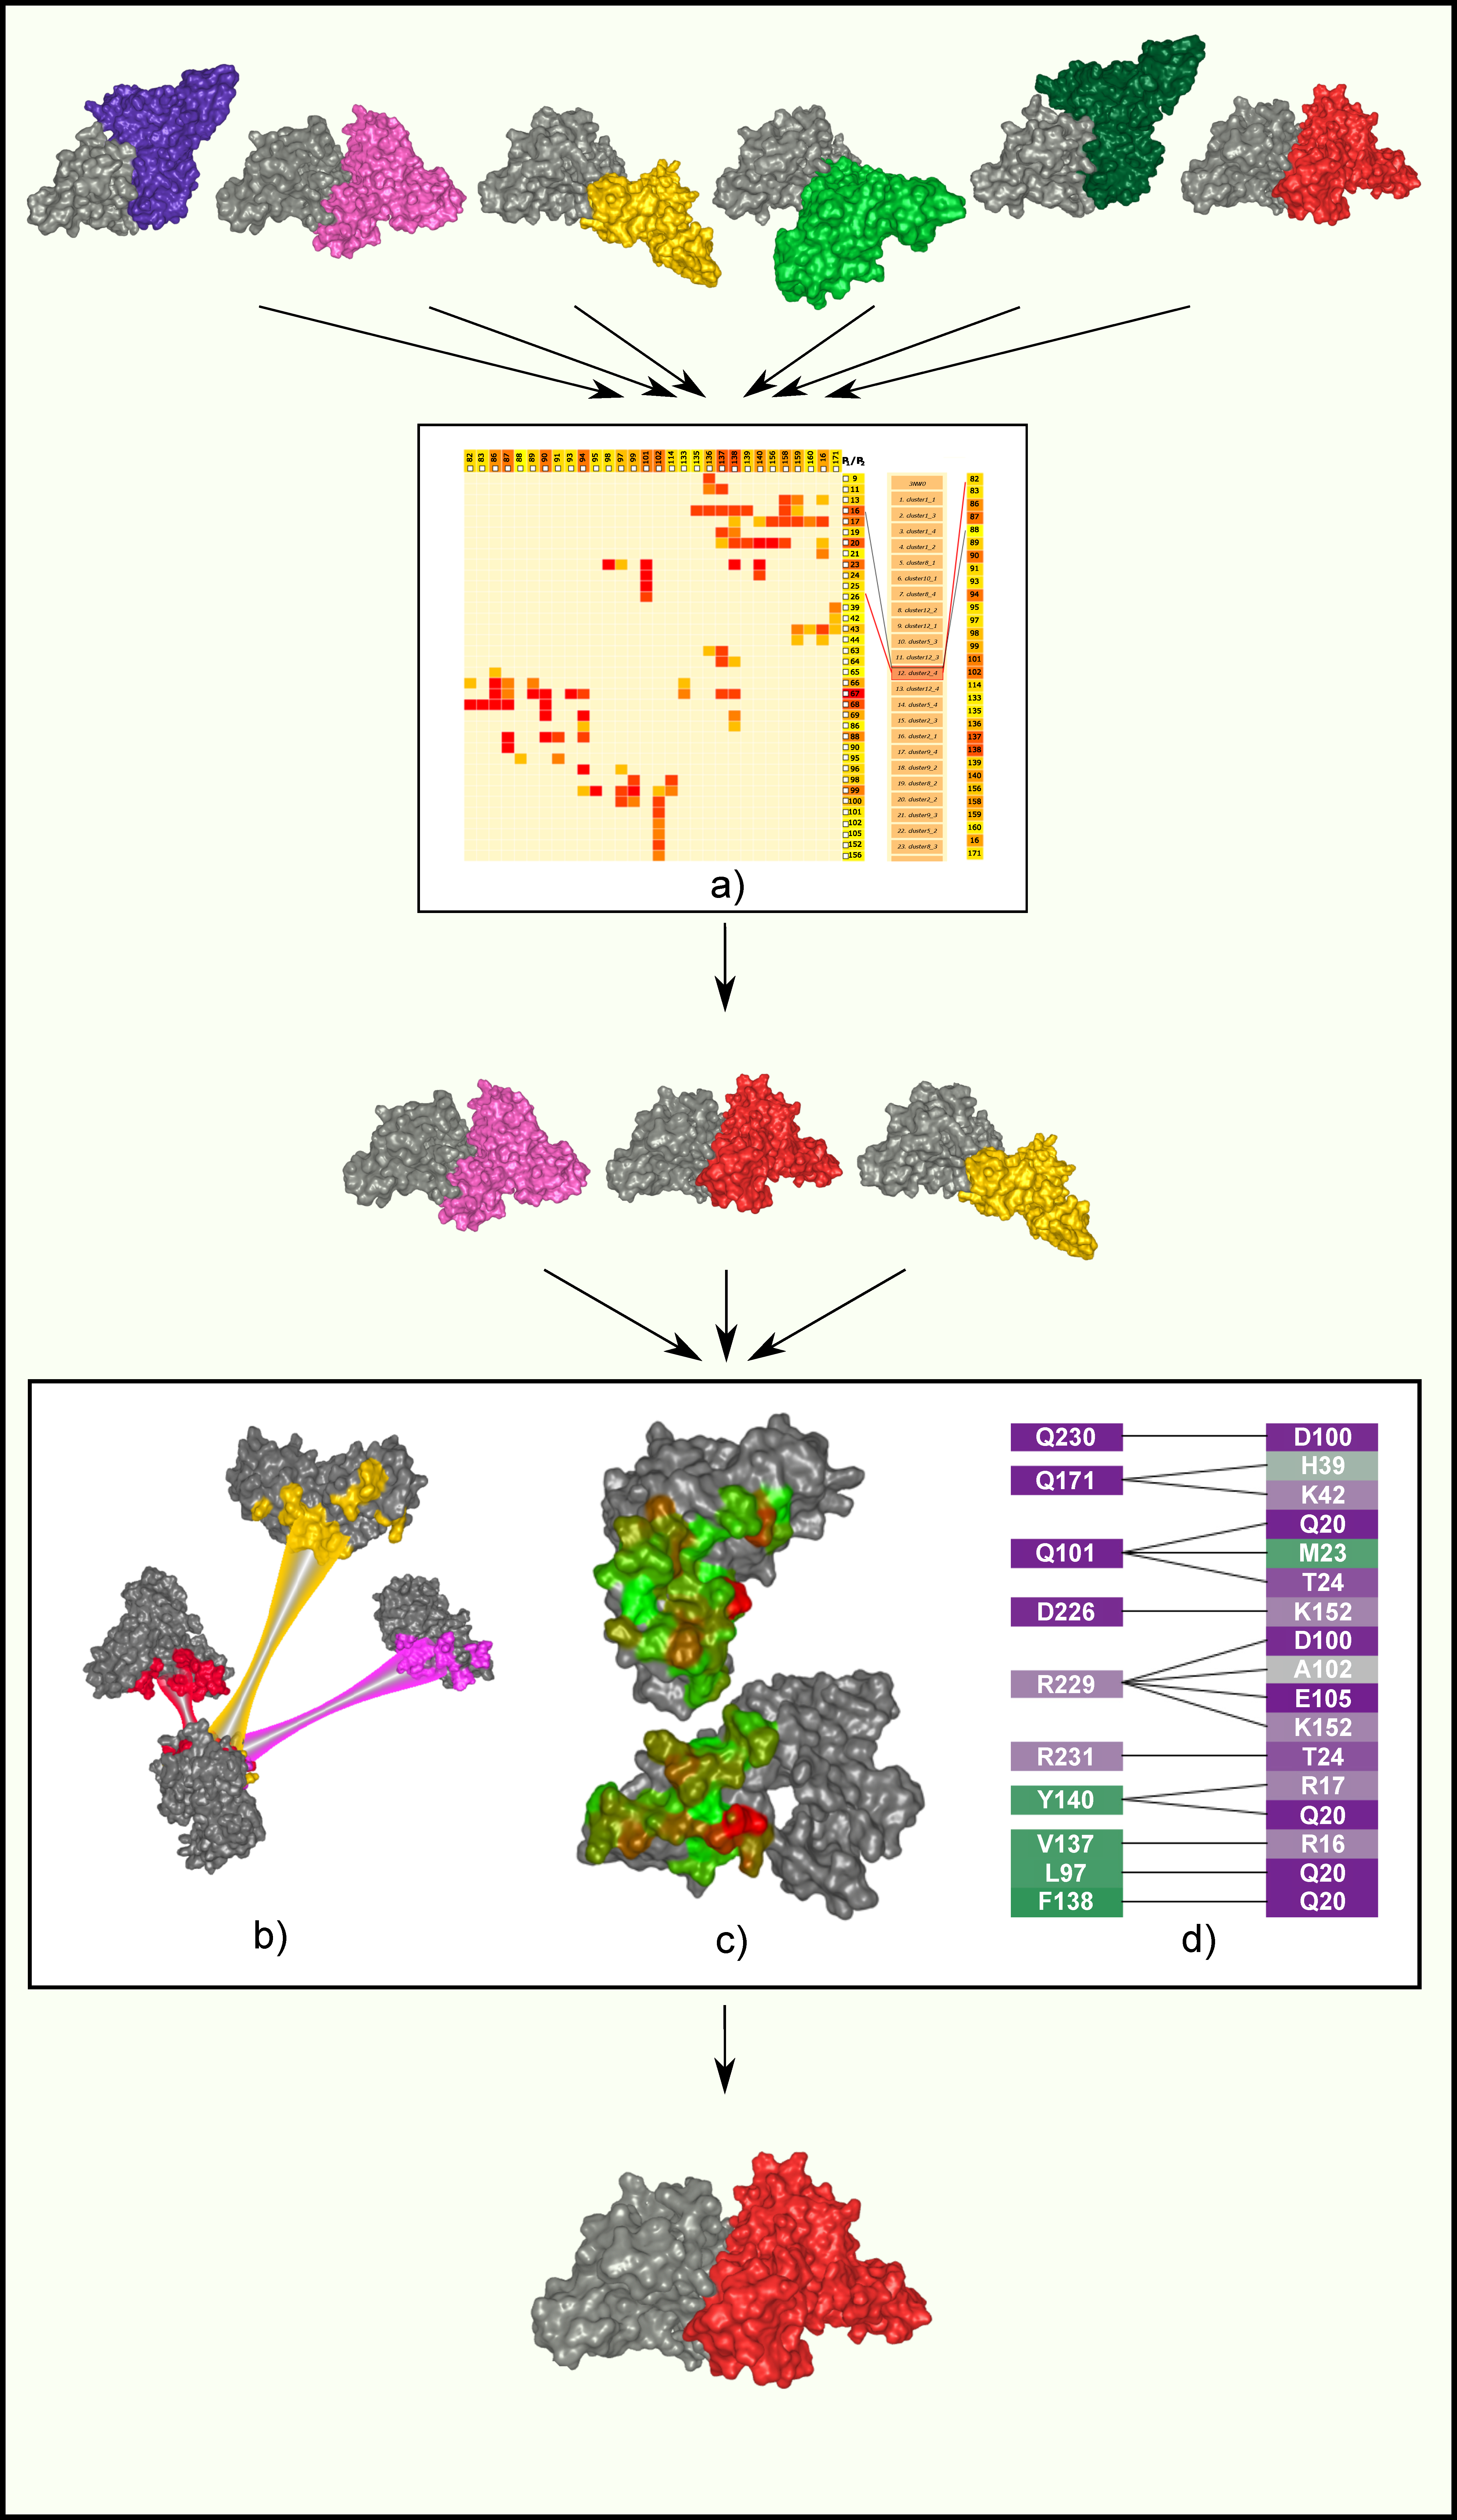
\includegraphics[width=0.9\columnwidth]{images/figure3.pdf}
  \caption{\csentence{Workflow overview.}
  The exploration process followed by the domain experts and our proposed supporting visualizations. (a) The \MatView represents an overview of all input configurations, obtained by one of the existing computational tools. (b) The \ExpView enables the user to explore the contact zones and their differences for a set of selected configurations. (c) The \OpBook animates the opening of a selected configuration. (d) The \CoZoListView supports the detailed comparison of the constitution of the contact zones of selected configurations.}
  \label{fig:workflow}
\end{figure}

\begin{figure}[h!]
  \centering
  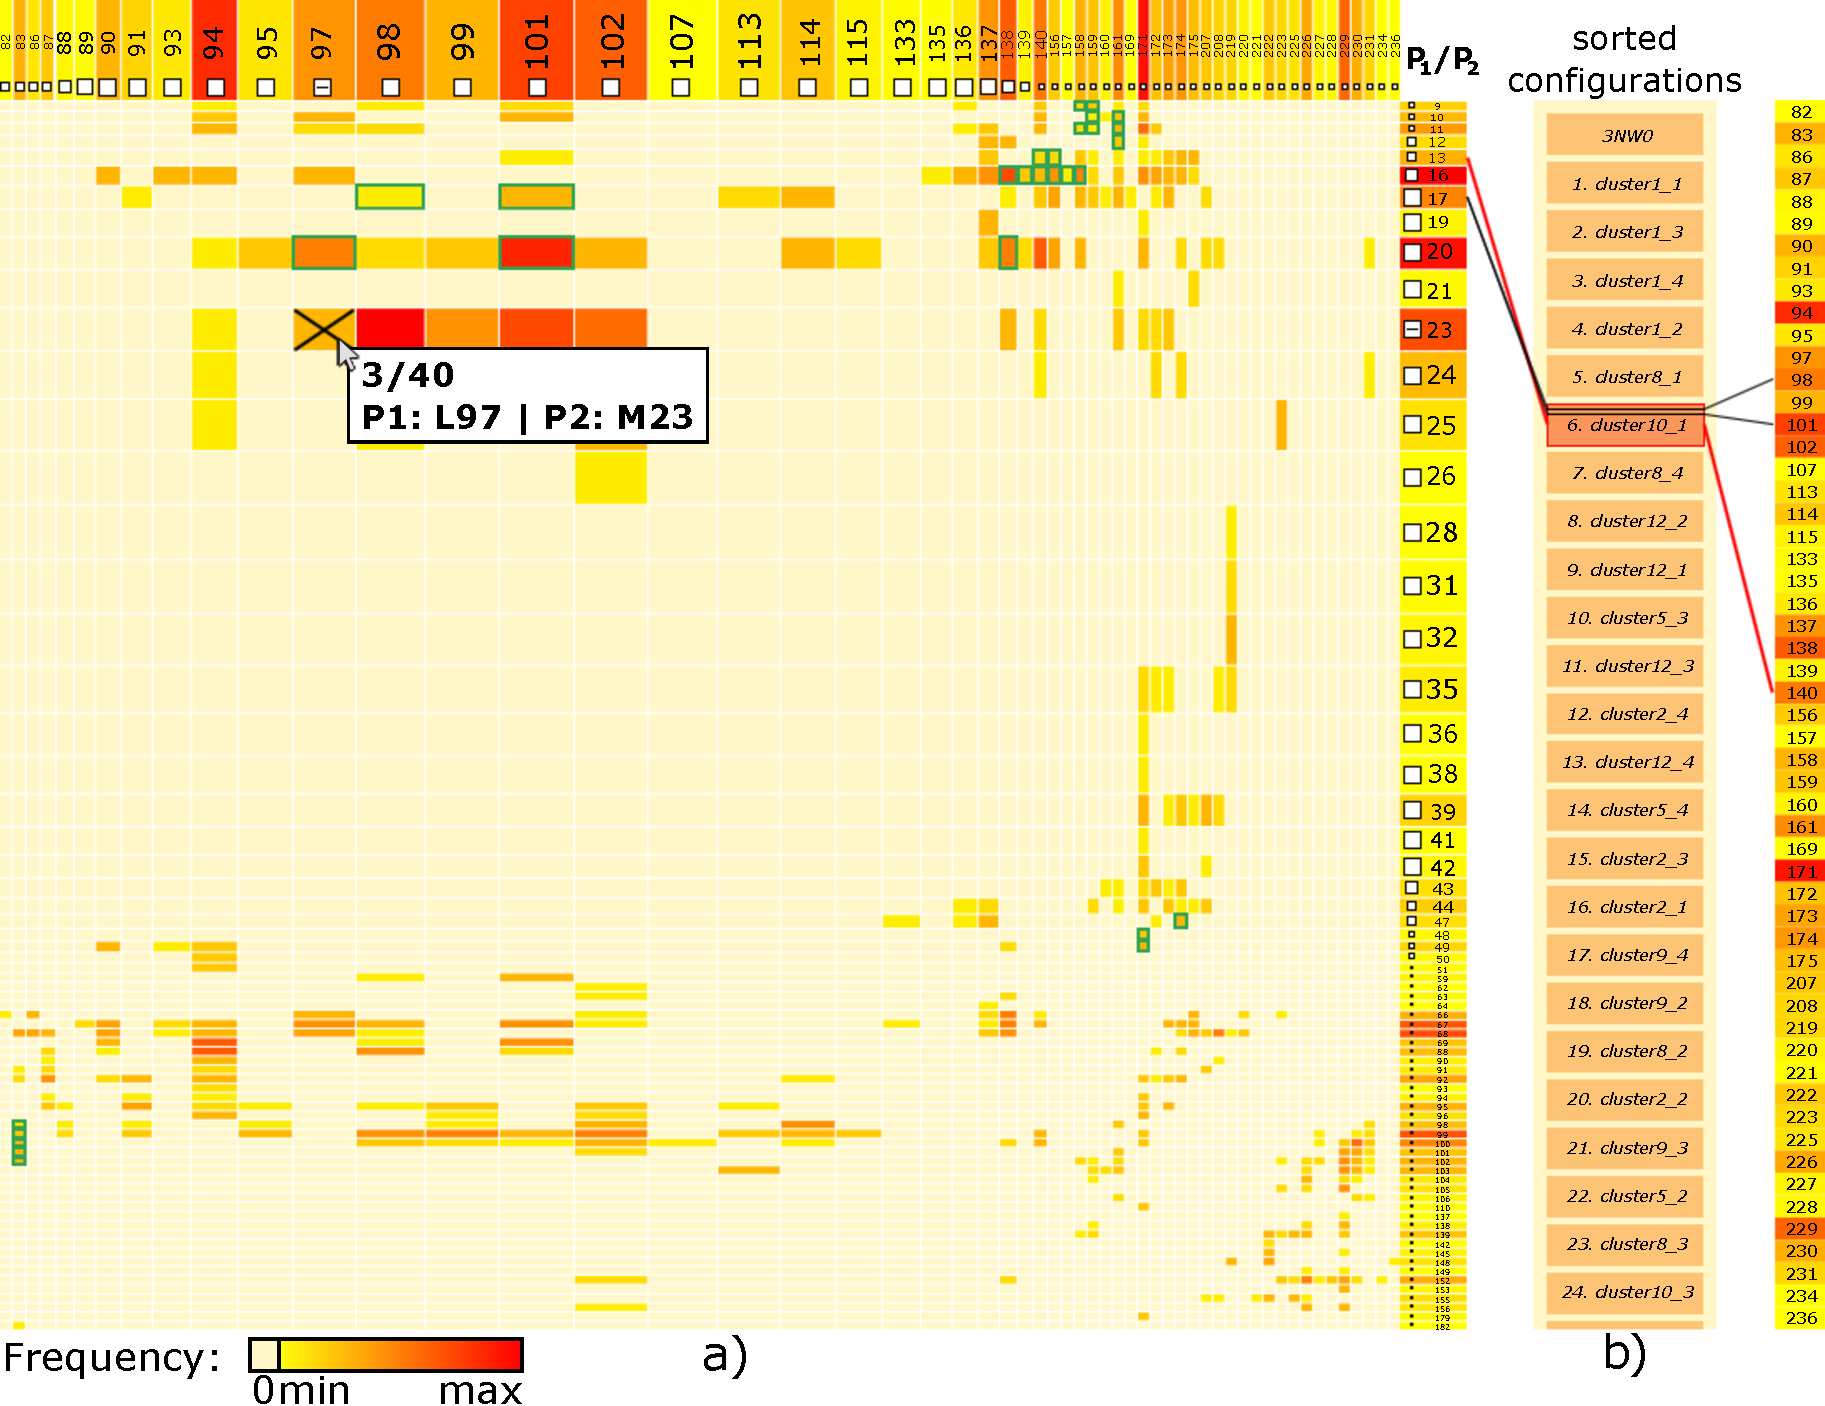
\includegraphics[width=0.9\columnwidth]{images/figure4.pdf}
  \caption{\csentence{Matrix view for the exploration and filtering of the input configurations.}
  (a) \MatView showing the aggregated information about the presence of mutually interacting amino acids in all configurations. Horizontal and vertical axes contain the lists of amino acids in the contact zones of the interacting proteins $P_1$ and $P_2$. (b) The side view shows individual configurations sorted according to their similarity to the primary configuration. The interaction with the side view enables to gain more detailed information about the configurations and their interacting amino acids. The central part of the side view consists of a scrollable list of individual configurations. The vertical list of amino acids (the rightmost column) is the same list as the one on the horizontal axis. The configuration in focus contains one polyline connecting those two amino acids from the contact zone which are the closest ones (red lines). The remaining interactions between amino acids are marked with black polylines. The green borders of some matrix cells represent the pairs which are present in the configuration selected in the side view. The selected cells are marked with a cross. It is possible to enlarge a selected row and column using an interactive lens.}
  \label{fig:matrixlens}
\end{figure}


%\begin{figure}[hbt]
%  \centering
%  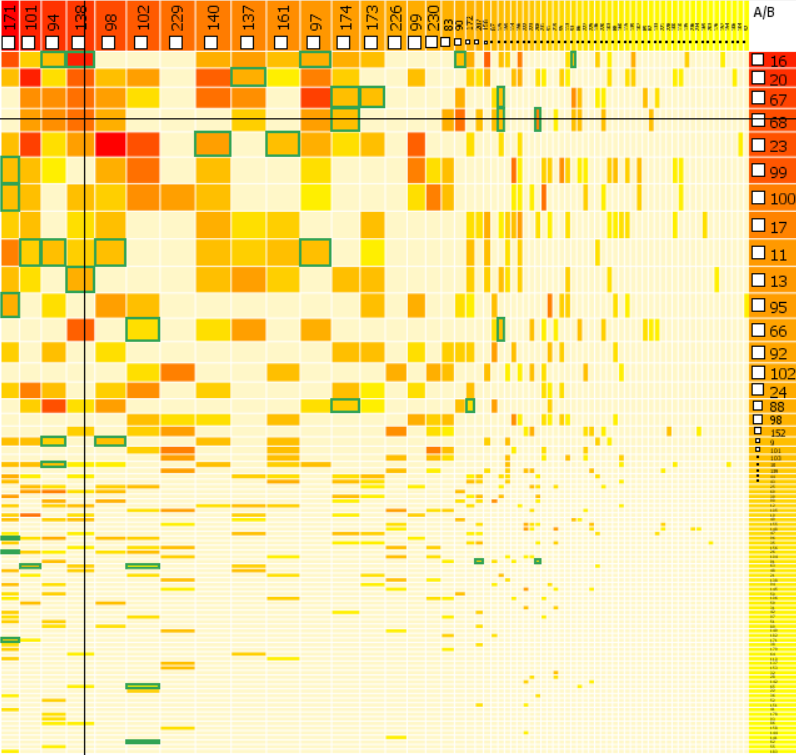
\includegraphics[width=0.8\columnwidth]{images/sort2.png}
%  \caption{\MatView sorted according to the frequency of occurrence of the amino acids in all configurations. Green borders of some matrix cells represent the pairs which are present in some of the configurations (selected in the InCo lens view). Selected cells are marked with a cross. Table lens technique enables to enlarge a selected row and column.}
%  \label{fig:sort}
%\end{figure}


\begin{figure}[h!]
    \centering
    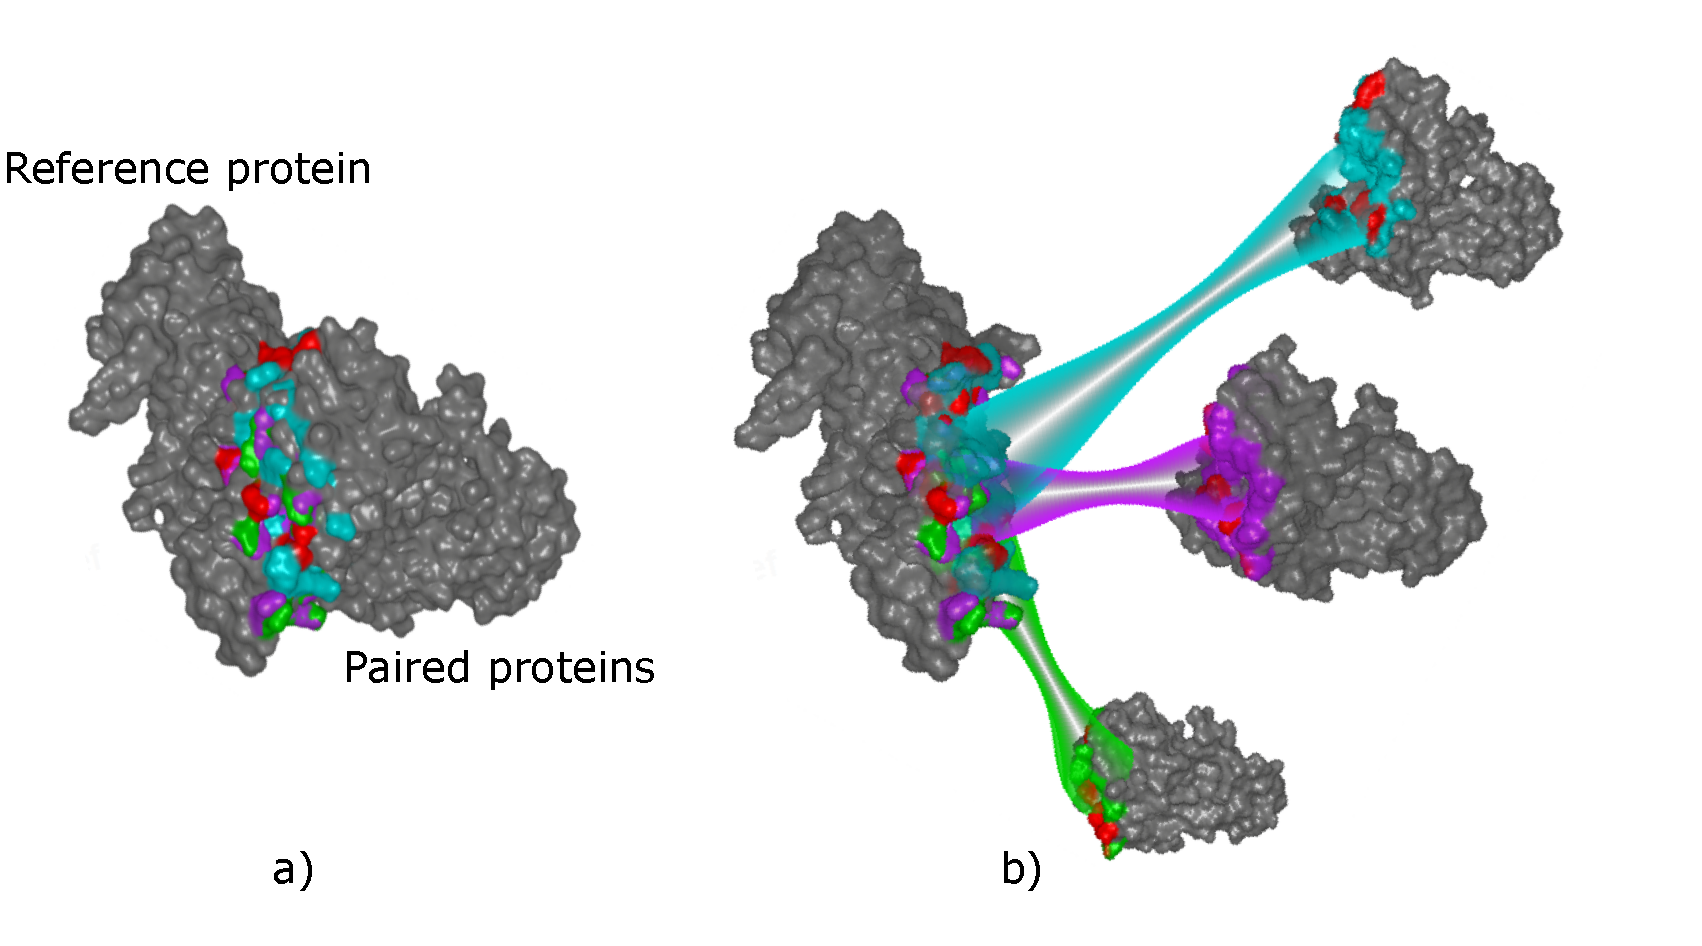
\includegraphics[width=0.9\columnwidth]{images/figure5.pdf}
    \caption{\csentence{Exploded view.}
    (a) Three configurations represented by surfaces with highlighted contact zones. (b) Aligned configurations. Their contact zones are almost completely occluded. (c) \ExpView of these configurations. A different color is used for each contact zone.}
	\label{fig:case12}
\end{figure}

\begin{figure}[h!]
  \centering
  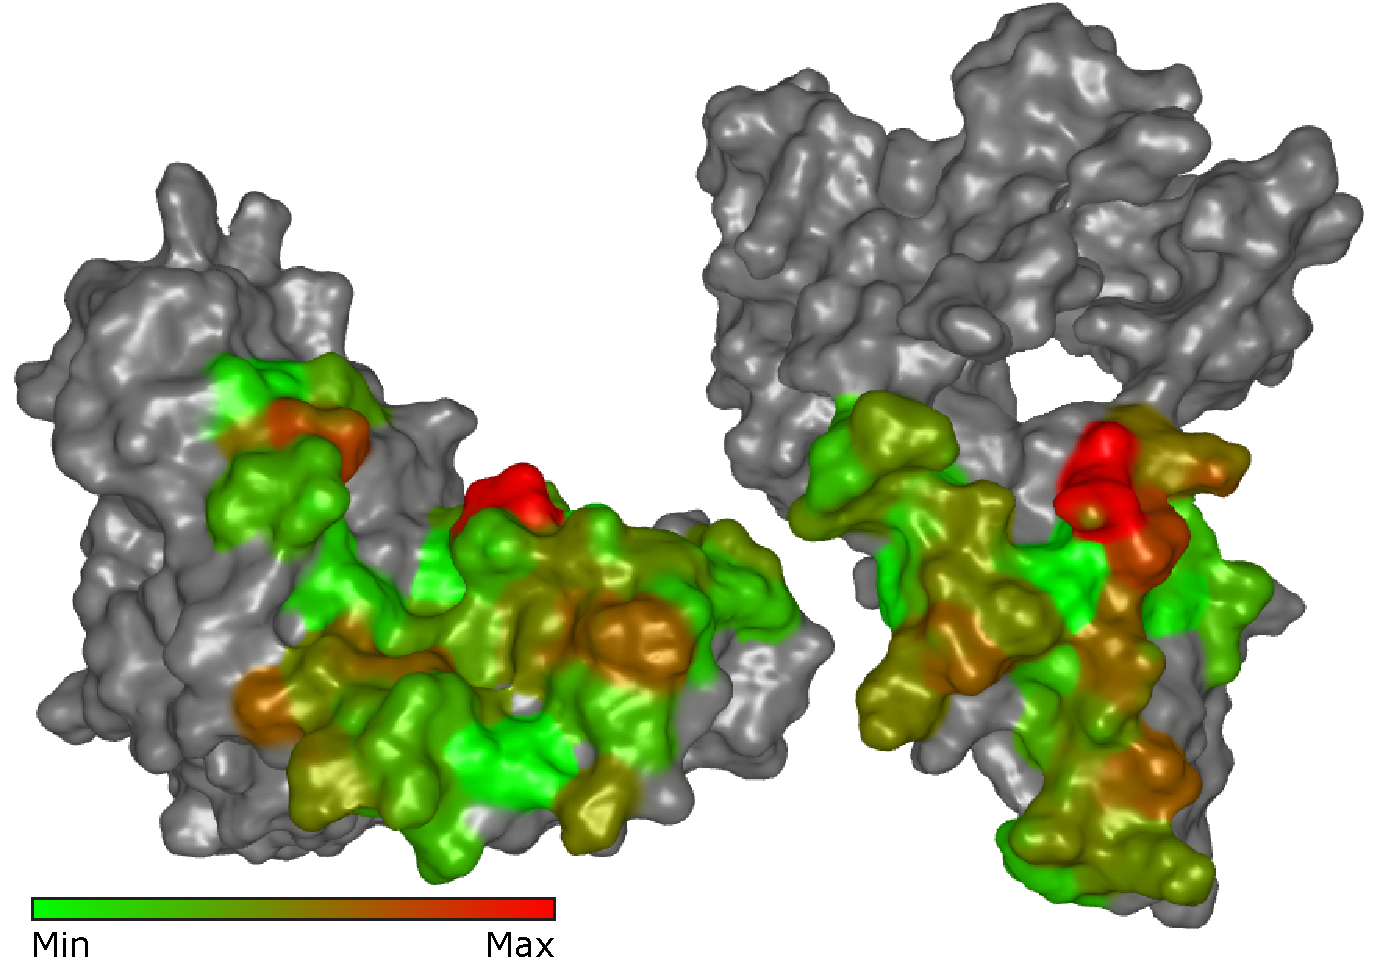
\includegraphics[width=0.9\columnwidth]{images/figure6.pdf}
  \caption{\csentence{\OpBook.} \OpBook enables the user to explore the contact zones between the interacting proteins simultaneously. On the left there is the reference protein and on the right there is the corresponding paired protein. The surface of the contact zones can be color-coded according to different criteria. Here the color represents the distance between the pairs of amino acids (red represents the closest ones, green the most distant ones).}
  \label{fig:book}
\end{figure}

\begin{figure}[h!]
    \centering
  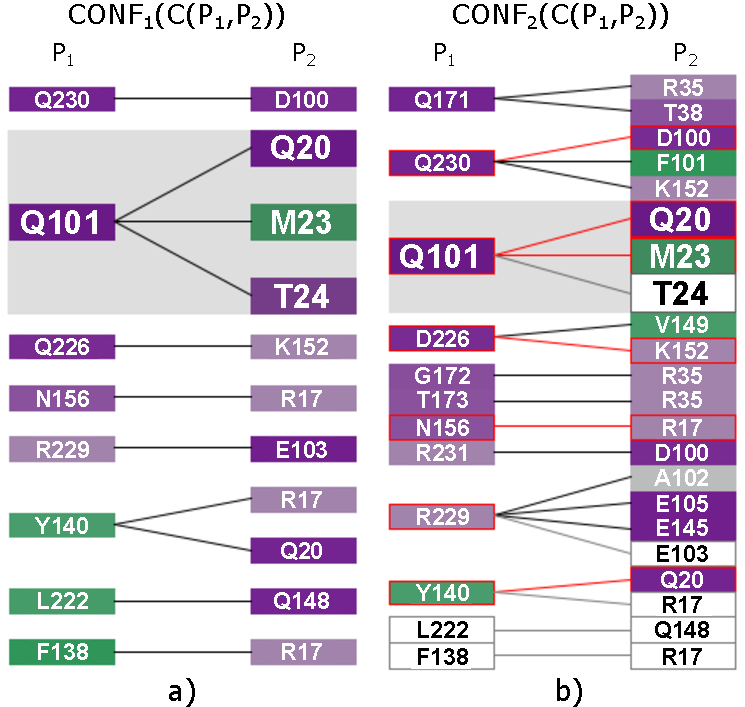
\includegraphics[width=0.7\columnwidth]{images/figure7.pdf}
    \caption{\csentence{\CoZoListView.} This view shows the comparison of one configuration, the primary one (a), with another selected configuration (b). For better comparison of configurations, the corresponding amino acids are interactively highlighted by zooming in. The view is sorted (and colored) according to hydrophobicity of the amino acids in the $P_1$ protein. Red color indicates the matches between the contact zone amino acids of the primary and the compared configuration. White rectangles indicate amino acids that are present in the primary configuration but are missing in the compared one.}
  \label{fig:list}
\end{figure}


\begin{figure}[h!]
    \centering
  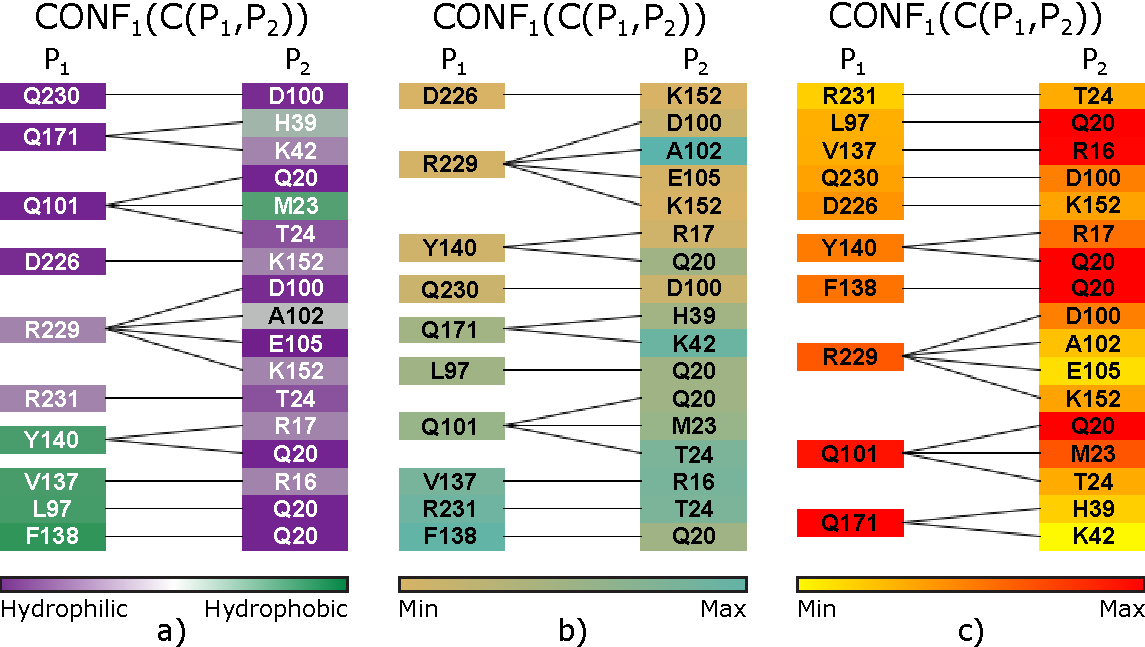
\includegraphics[width=0.9\columnwidth]{images/figure8.pdf}
    \caption{\csentence{The \CoZoListView and different properties.} Sorting of the \CoZoListView according to different properties of amino acids -- (a) hydrophobicity, (b) mutual distance, (c) frequency of occurrence of the pairs in all configurations.}
  \label{fig:sorting}
\end{figure}

\begin{figure}[h!]
    \centering
    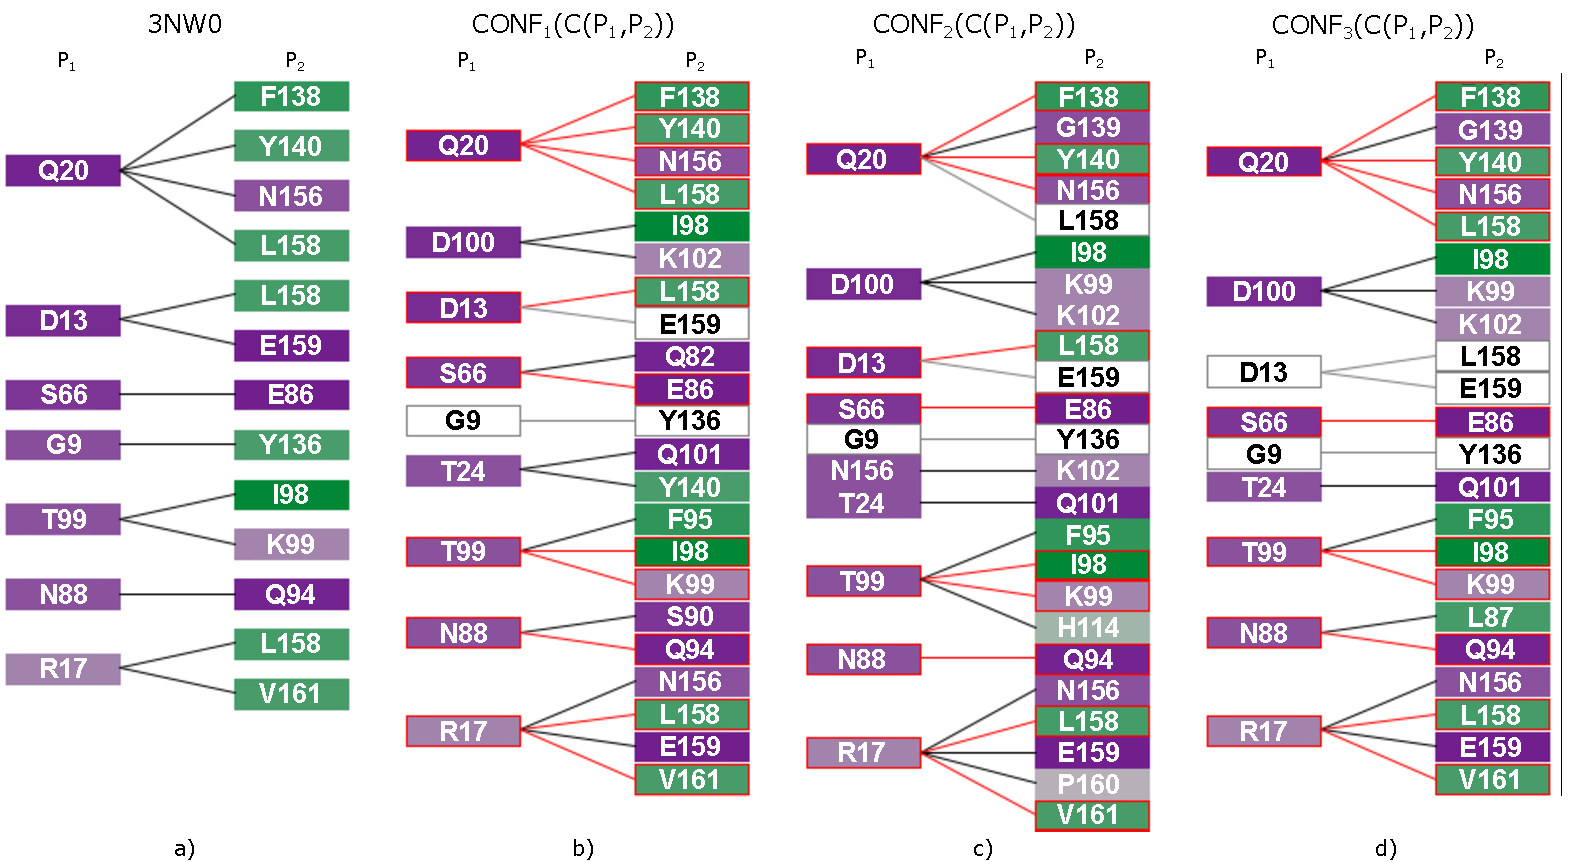
\includegraphics[width=0.9\columnwidth]{images/figure9.pdf}
    \caption{\csentence{Surface-Surface Interaction -- best HADDOCK configurations.} Example of four configurations represented by the juxtapositioned \CoZoListView. (a) Primary 3NW0 crystal structure, (b), (c), (d) three selected best-fit HADDOCK models. The lists are colored and sorted according to the hydrophobicity of the amino acids in the reference protein in each selected configuration.}
  \label{fig:case3}
\end{figure}

\begin{figure}[h!]
  \centering
  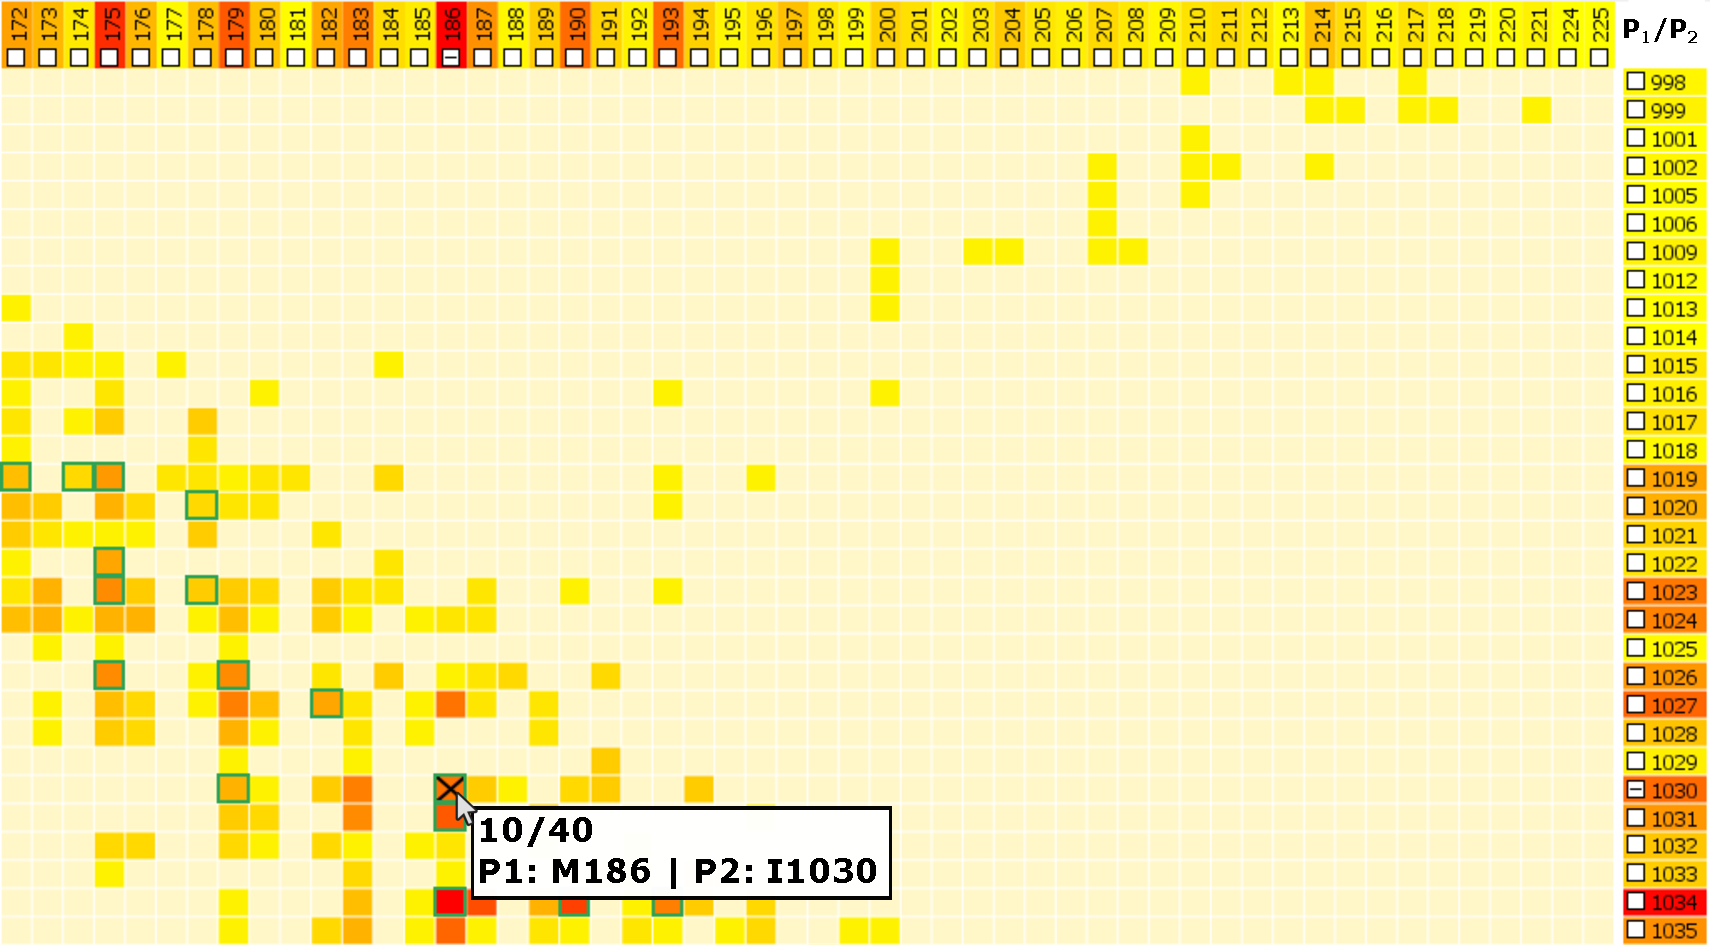
\includegraphics[width=0.9\columnwidth]{images/figure10.pdf}
  \caption{\csentence{Coiled-Coil Interaction -- the \MatView of interacting amino acids in all HADDOCK models.} The \MatView indicates that the selected pair of M186 and I1030 amino acids is present in 10 out of 40 loaded models.}
  \label{fig:coiled_haddock_mat}
\end{figure}

\begin{figure}[h!]
  \centering
  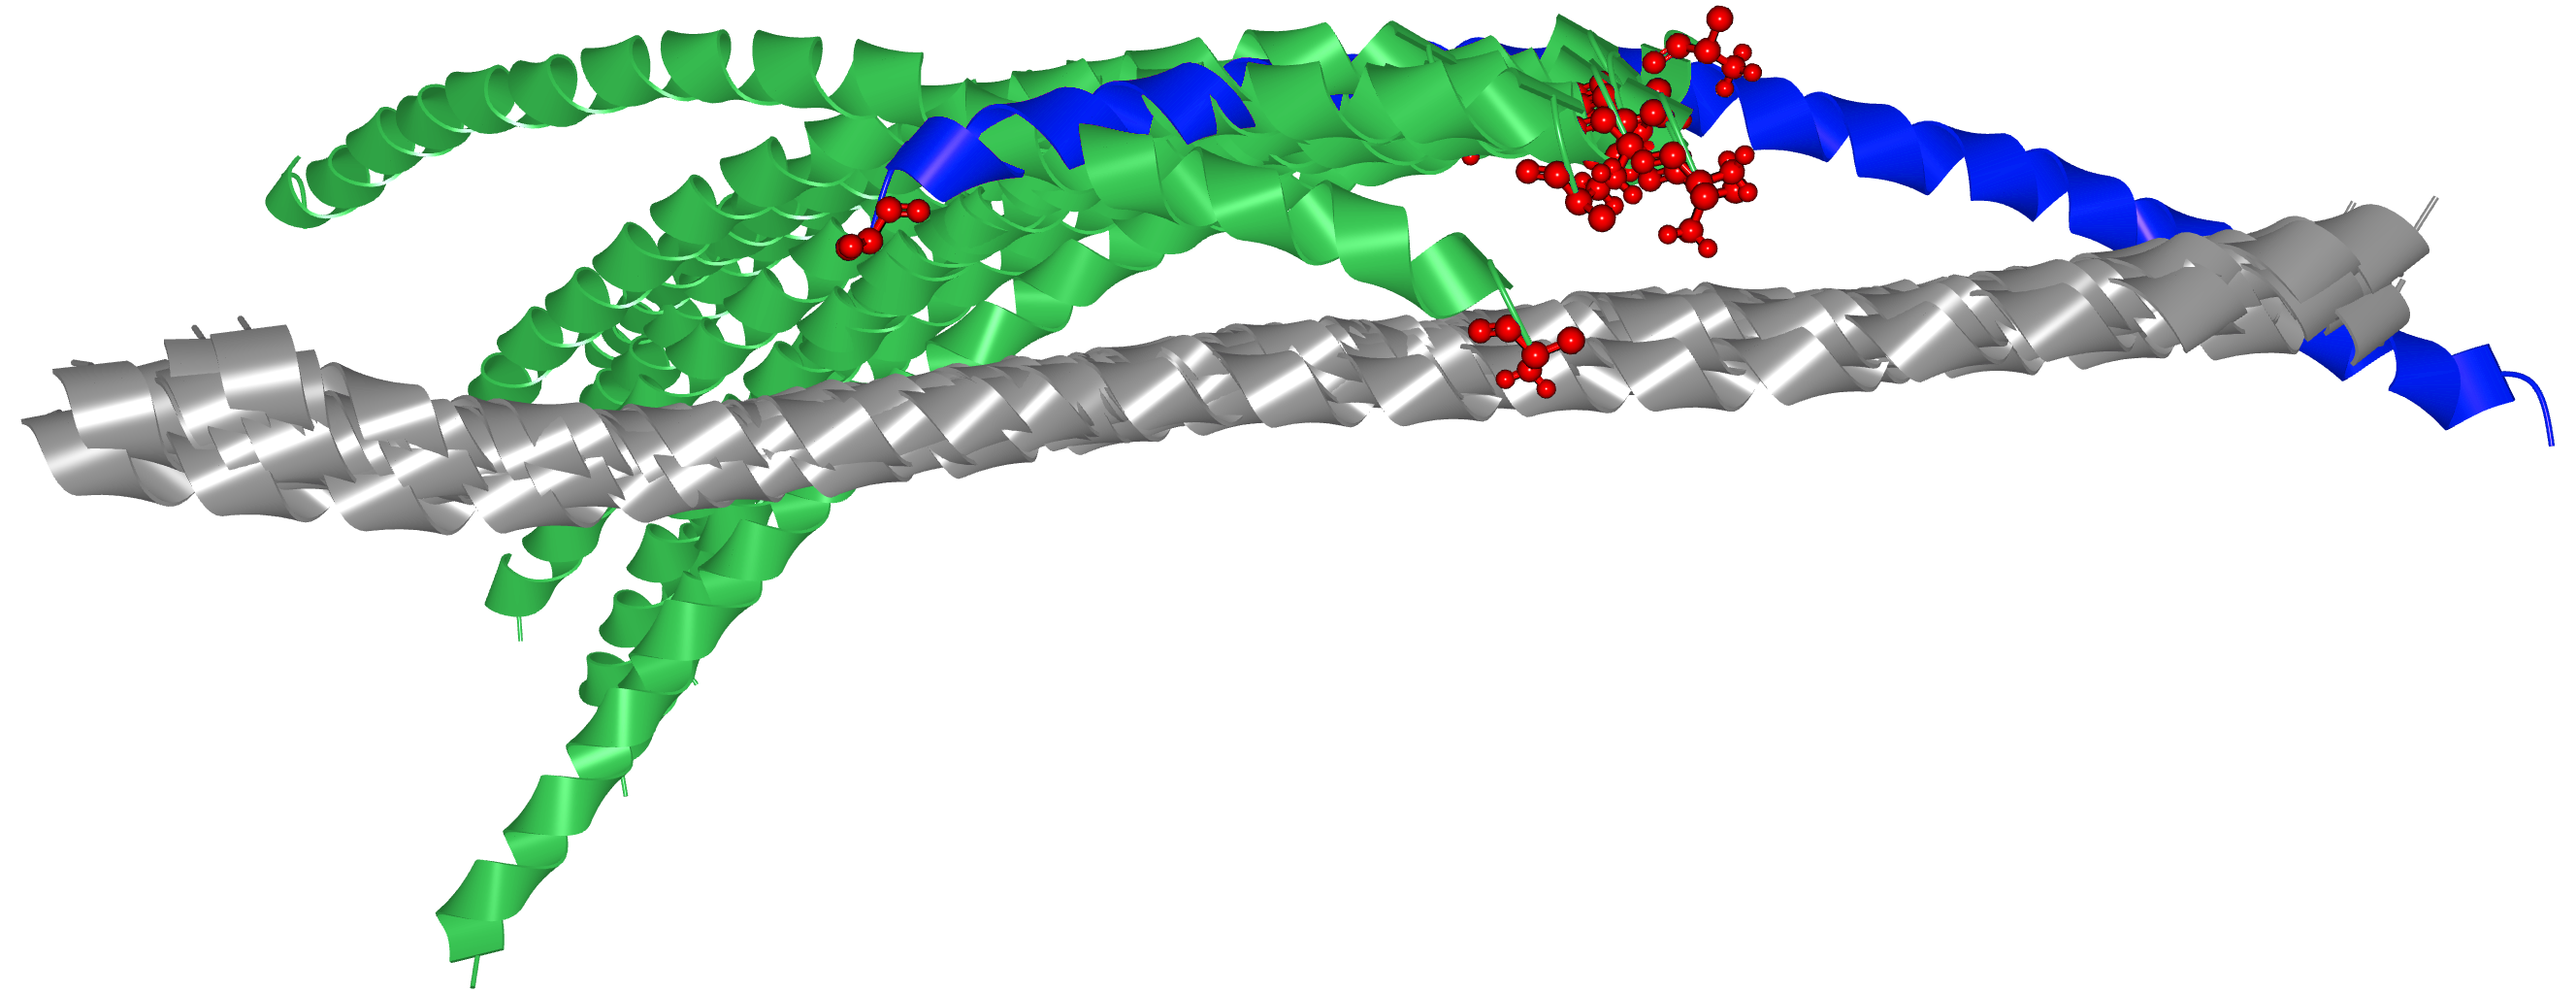
\includegraphics[width=0.9\columnwidth]{images/figure11.png}
  \caption{\csentence{Coiled-Coil Interaction -- 4UX3 crystal (blue) and 10 selected HADDOCK configurations (green).} The first A172 amino acid (red) is highlighted in all loaded structures. The opposite orientation of 4UX3 and HADDOCK models is clearly visible.}
  \label{fig:coiled_haddock}
\end{figure}

\begin{figure}[h!]
  \centering
  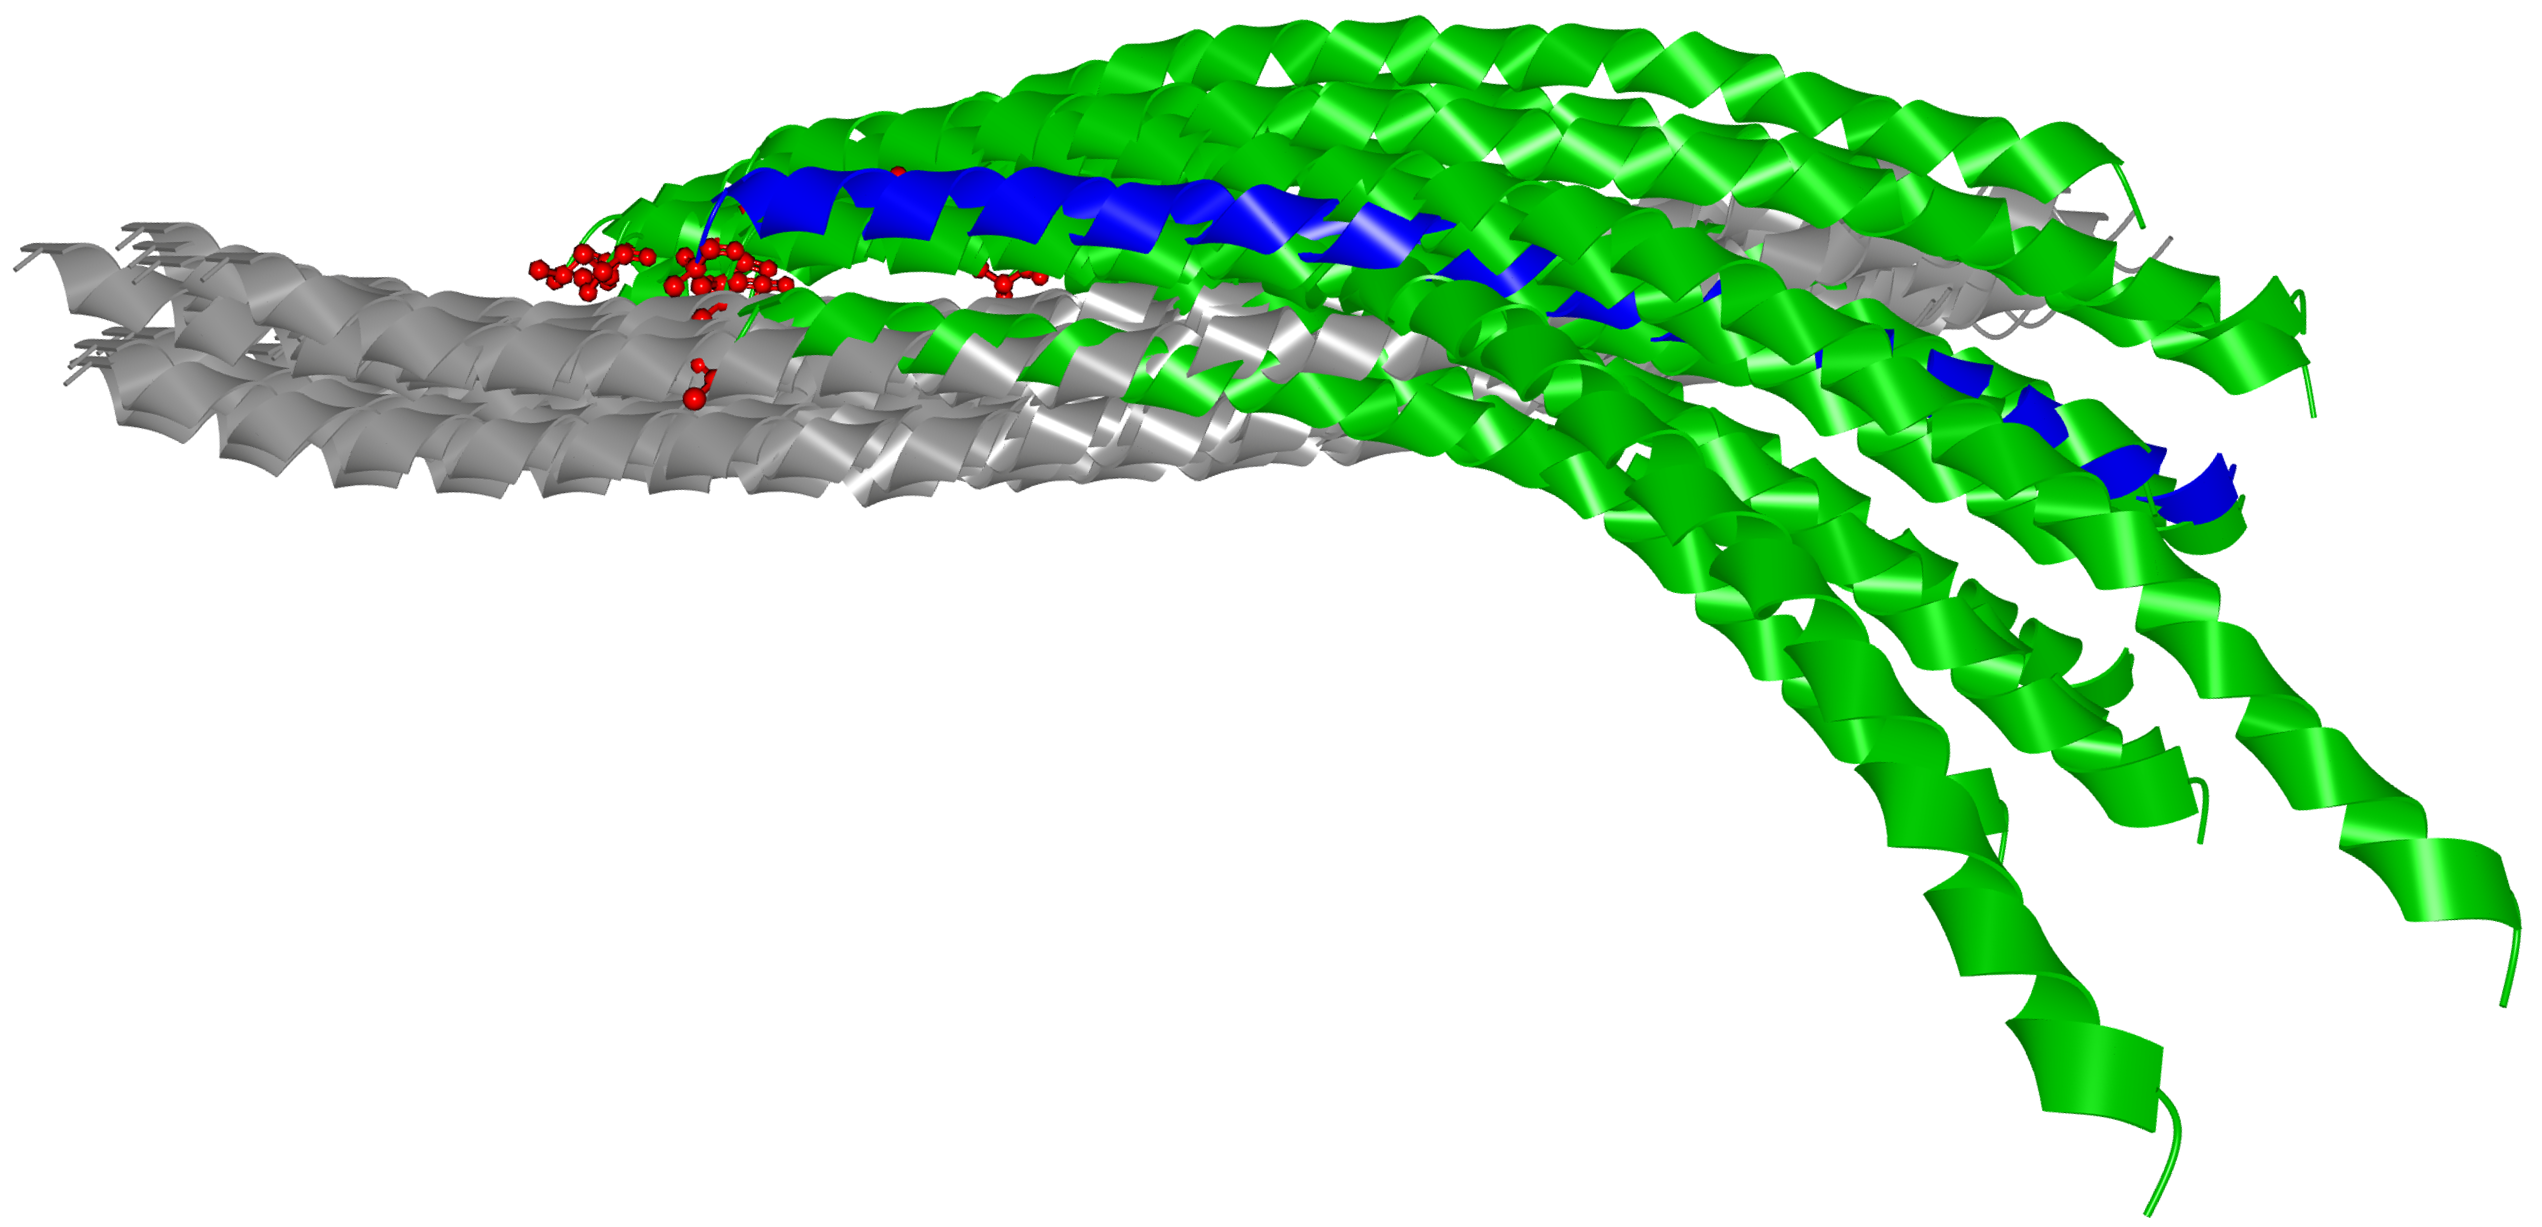
\includegraphics[width=0.9\columnwidth]{images/figure12.png}
  \caption{\csentence{Coiled-Coil Interaction -- 4UX3 crystal (blue) and 14 selected PyDock configurations (green).} In these PyDock configurations, all A172 amino acids (red balls and sticks) are positioned at the same side as in the crystal structure (blue).}
  \label{fig:selection2SMC3PyDock}
\end{figure}

\begin{figure}[h!]
    \centering
  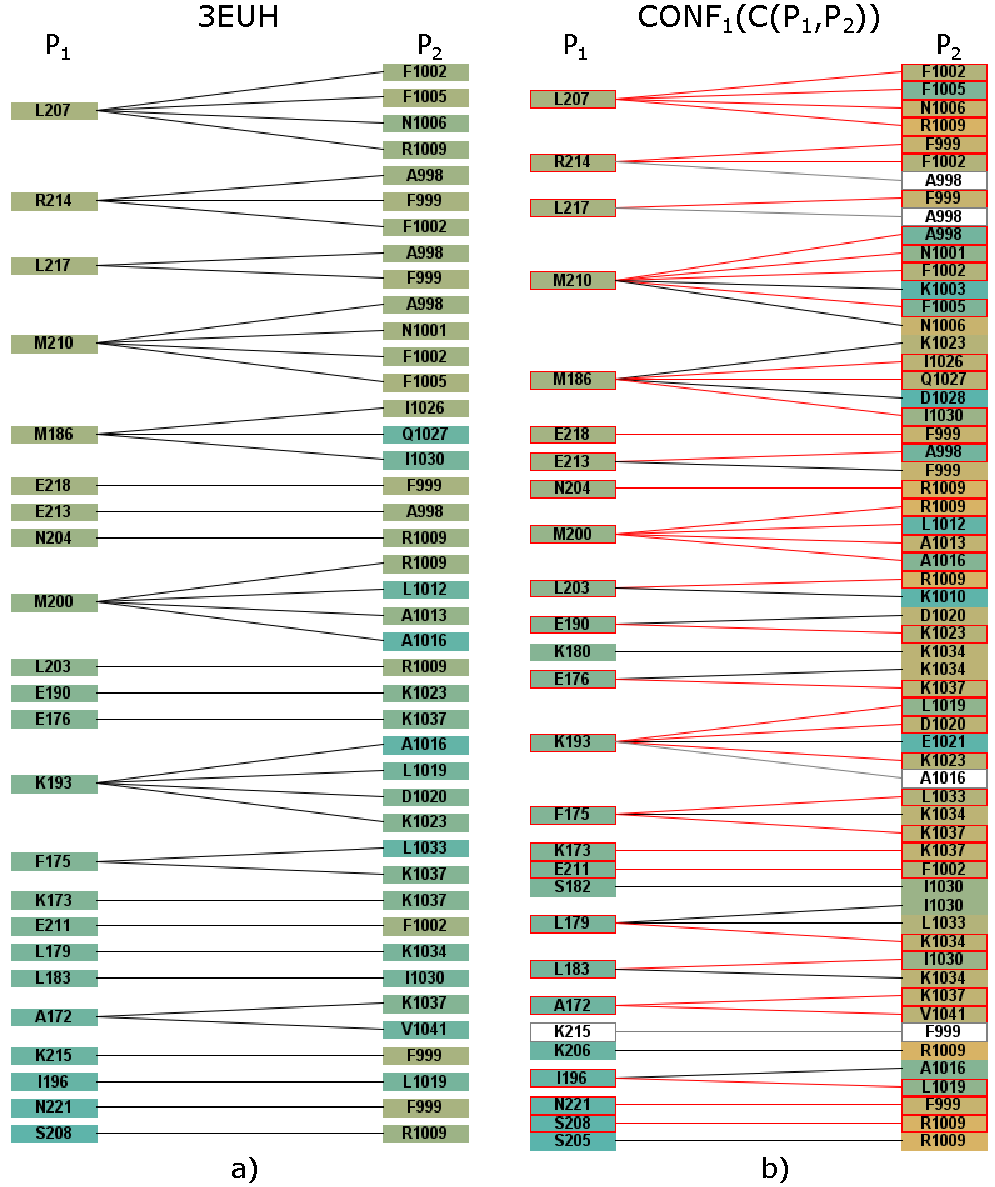
\includegraphics[width=0.9\columnwidth]{images/figure13.pdf}
    \caption{\csentence{Coiled-Coil Interaction -- best fitting PyDock configuration.} \CoZoList comparing the 4UX3 crystal with one best fit PyDock model with respect to the distances of amino acids.}
  \label{fig:coiled2}
\end{figure}

\begin{figure}[!h]
  \centering
  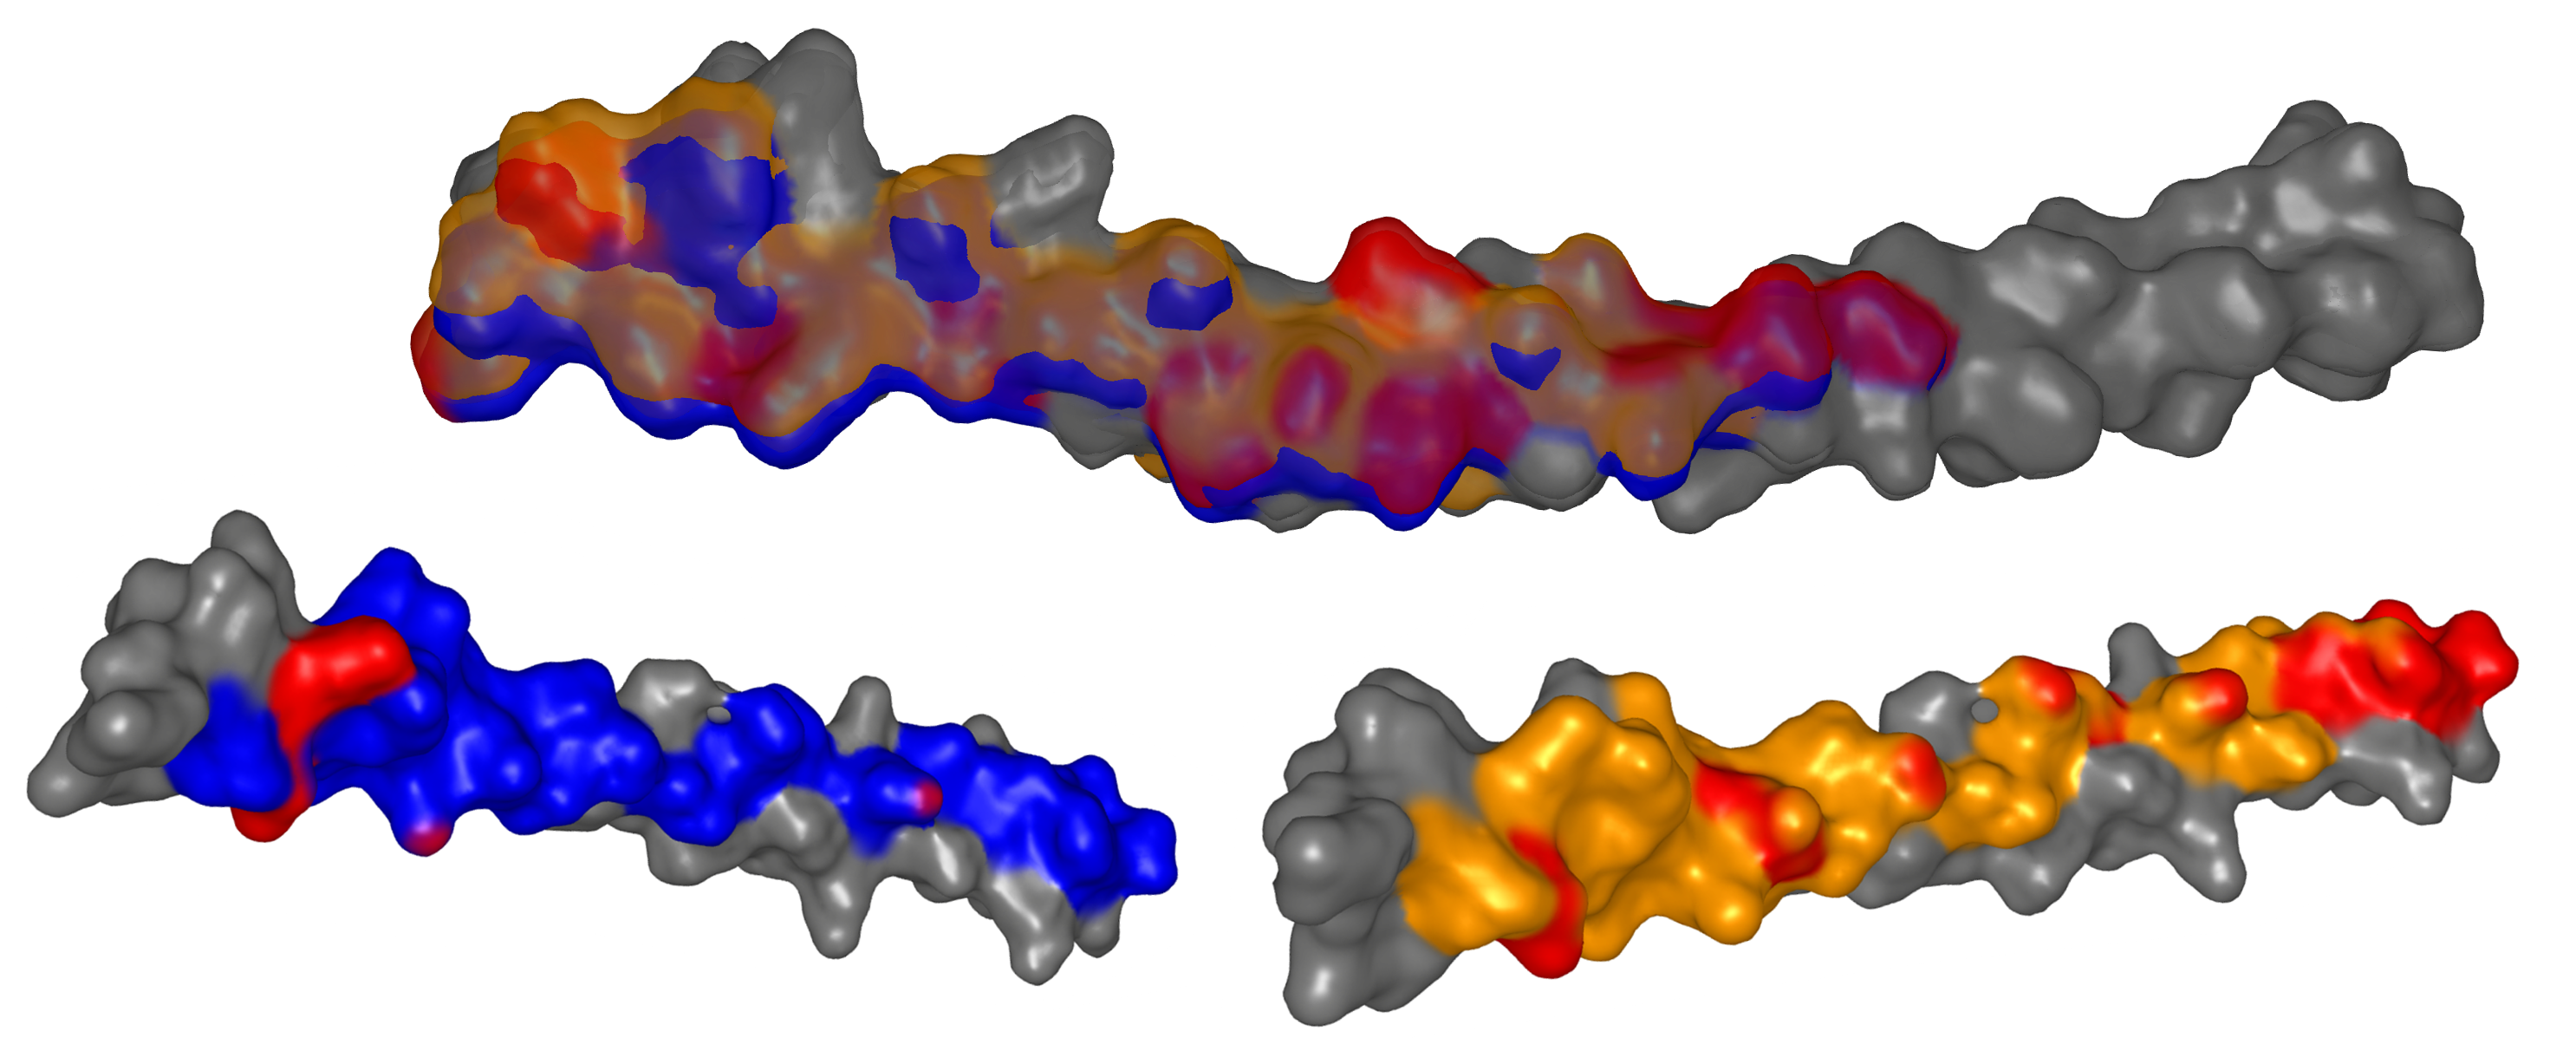
\includegraphics[width=0.9\columnwidth]{images/figure14.png}
  \caption{\csentence{Coiled-Coil Interaction -- best fitting PyDock configuration.} The \ExpView showing the contact zone of the best fitting PyDock model (orange) and the 4UX3 crystal (blue). On the top, the overlapping contact zones on the reference protein are shown. The bottom part of the image depicts the paired proteins.}
  \label{fig:selection_4_final_SMC3_PyDock}
\end{figure}

\begin{figure}[h!]
    \centering
    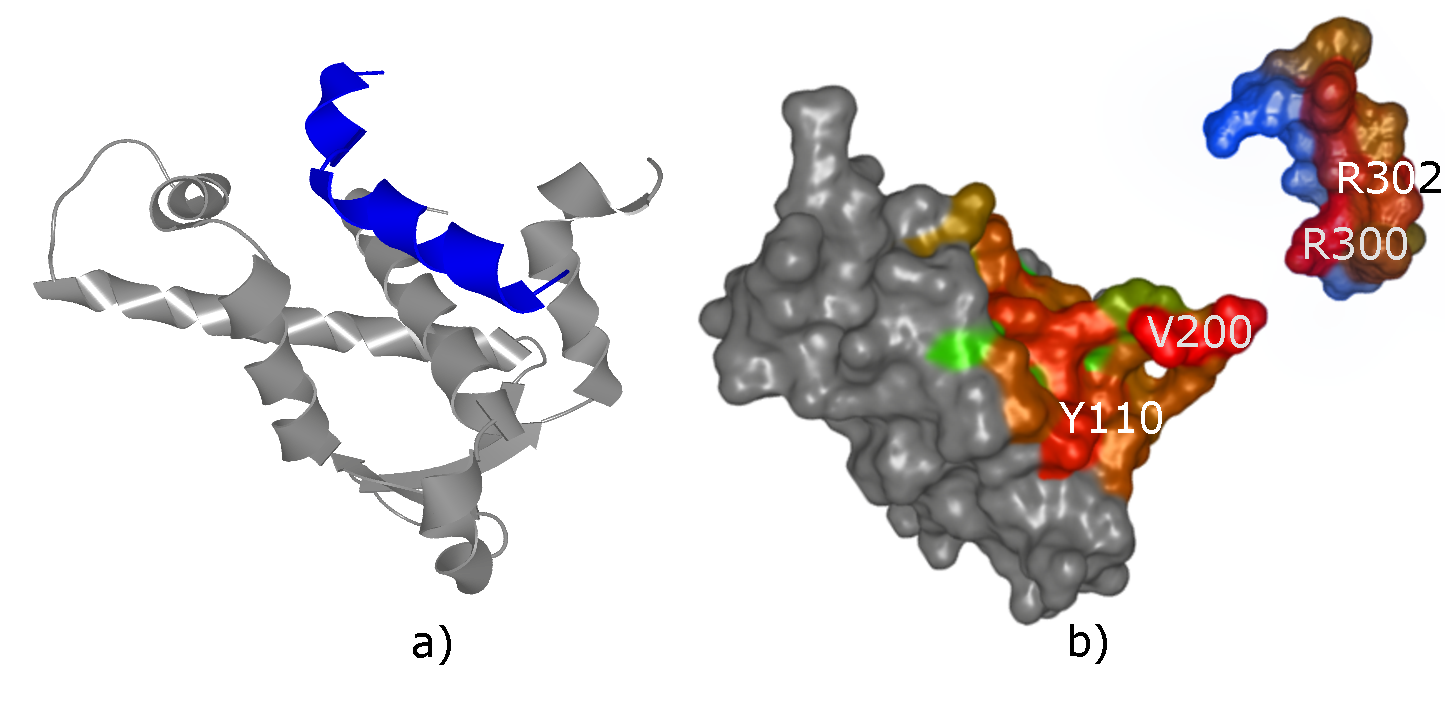
\includegraphics[width=0.9\columnwidth]{images/figure15.pdf}
    \caption{\csentence{Pocket-String Interaction -- 3EUH crystal structure.}(a) 3EUH crystal structure consisting of the domain containing the pocket (grey) and the helical fragment of the second domain (blue), shown using the cartoon representation. (b) The same structure shown with the \OpBook. The contact zones are colored according to the distance between the interacting amino acids and the labels of the two closest pairs are shown.}
  \label{fig:MukEF_crystal_3EUH_selected}
\end{figure}

\begin{figure}[h!]
    \centering
    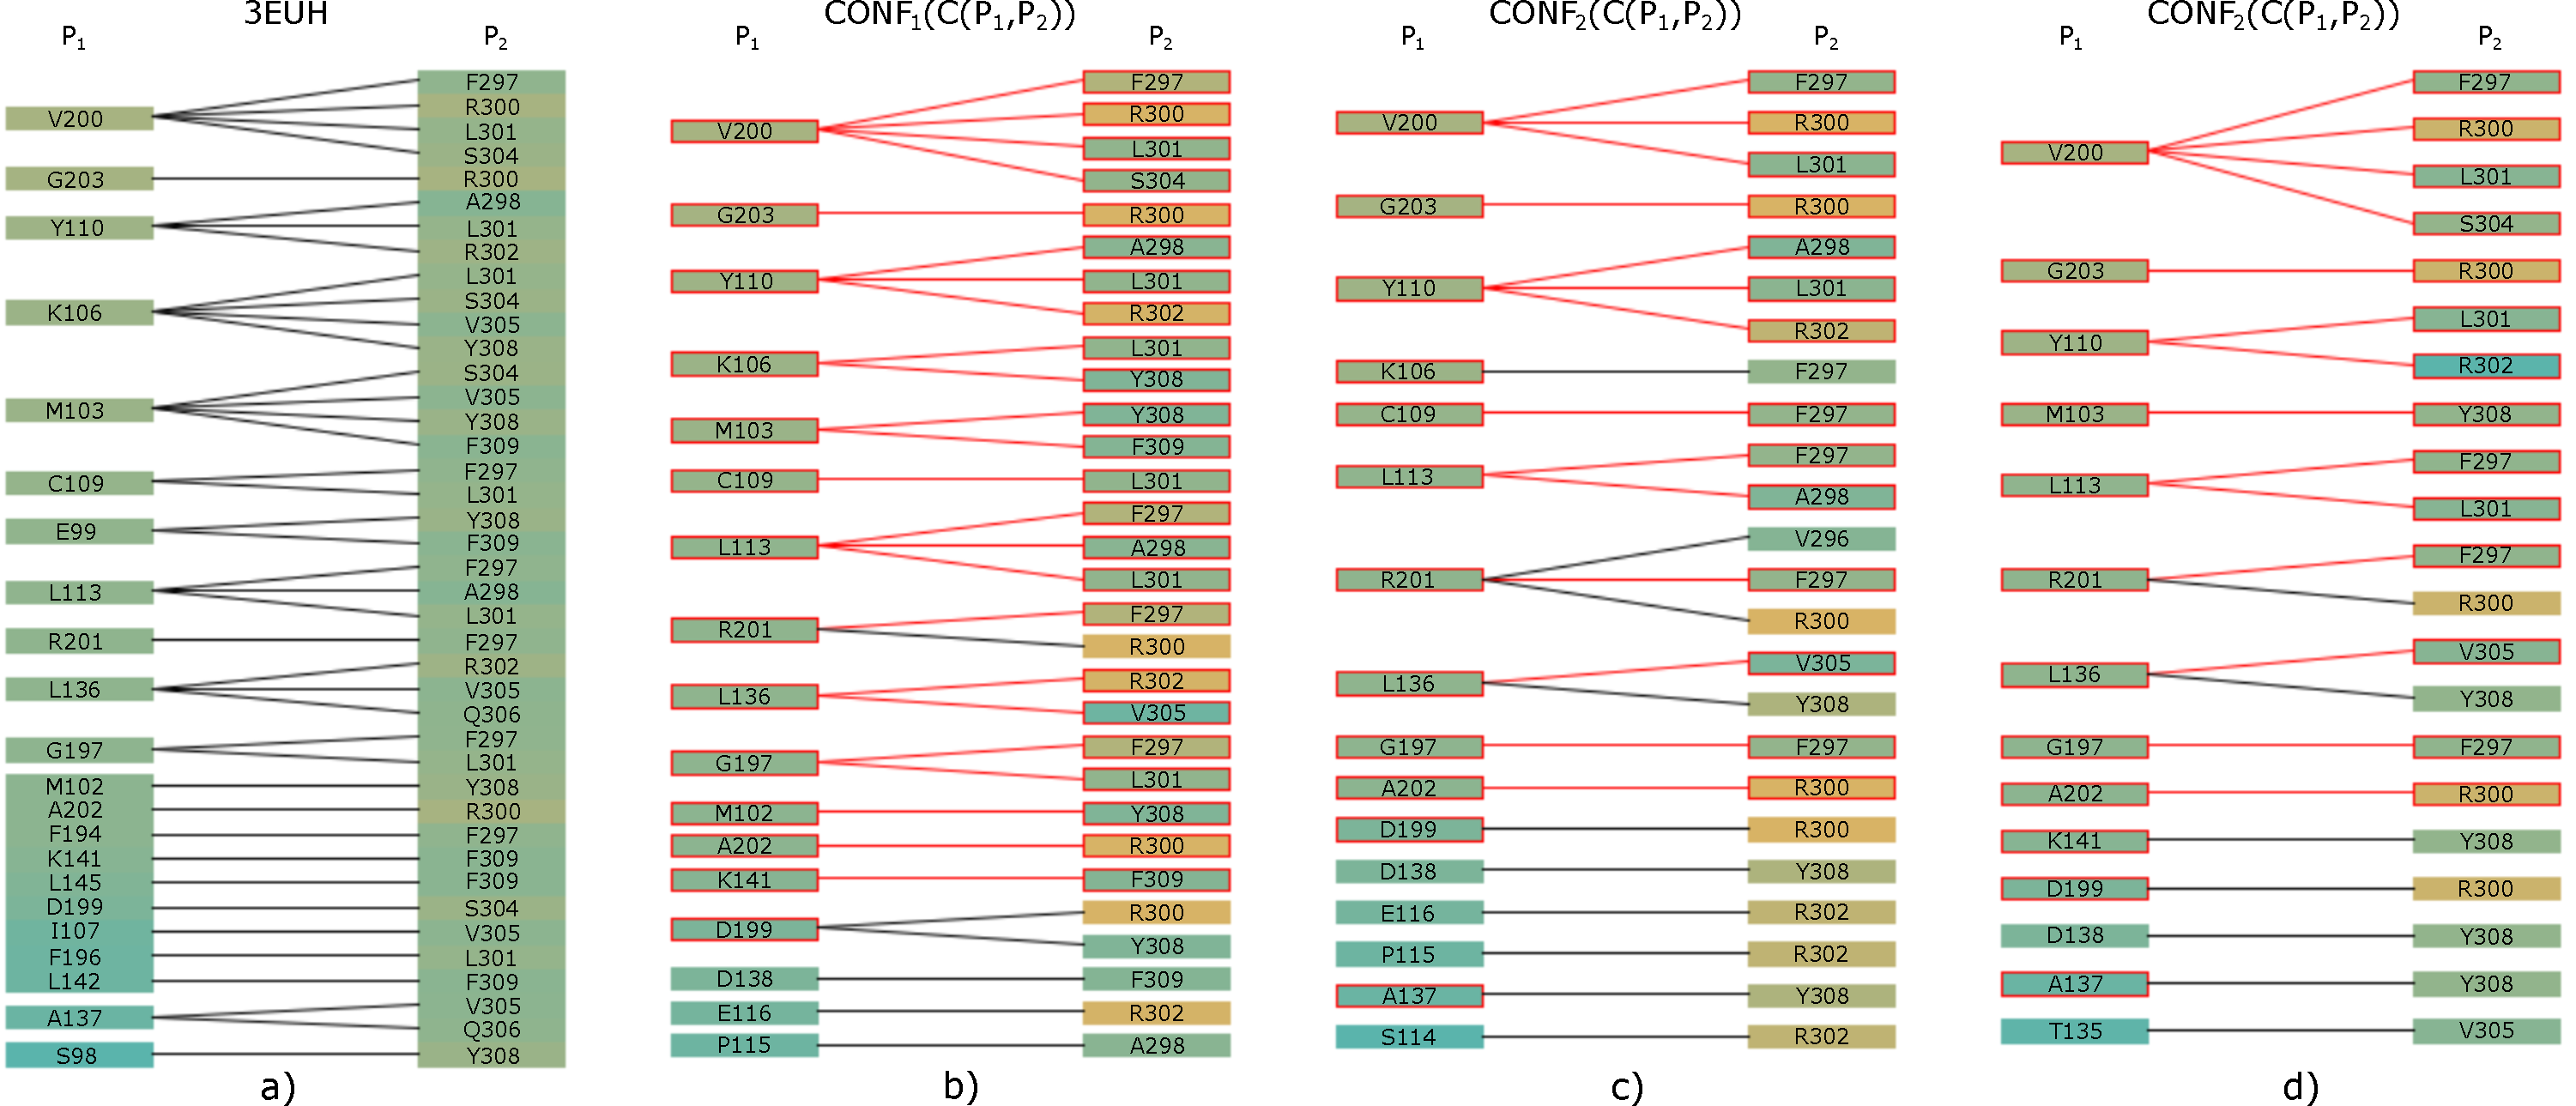
\includegraphics[width=0.9\columnwidth]{images/figure16.pdf}
    \caption{\csentence{Pocket-String Interaction -- best HADDOCK configurations.} \CoZoLists of the selected HADDOCK configurations sorted according to the distance of the amino acids. (a) The primary 3EUH crystal structure, (b), (c), (d) three selected HADDOCK models. The sorting shows that the V200-R300 pair is one of the closest ones in the crystal as well as in all selected models.}
  \label{fig:list_pocket_string}
\end{figure}

\begin{figure}[h!]
  \centering
  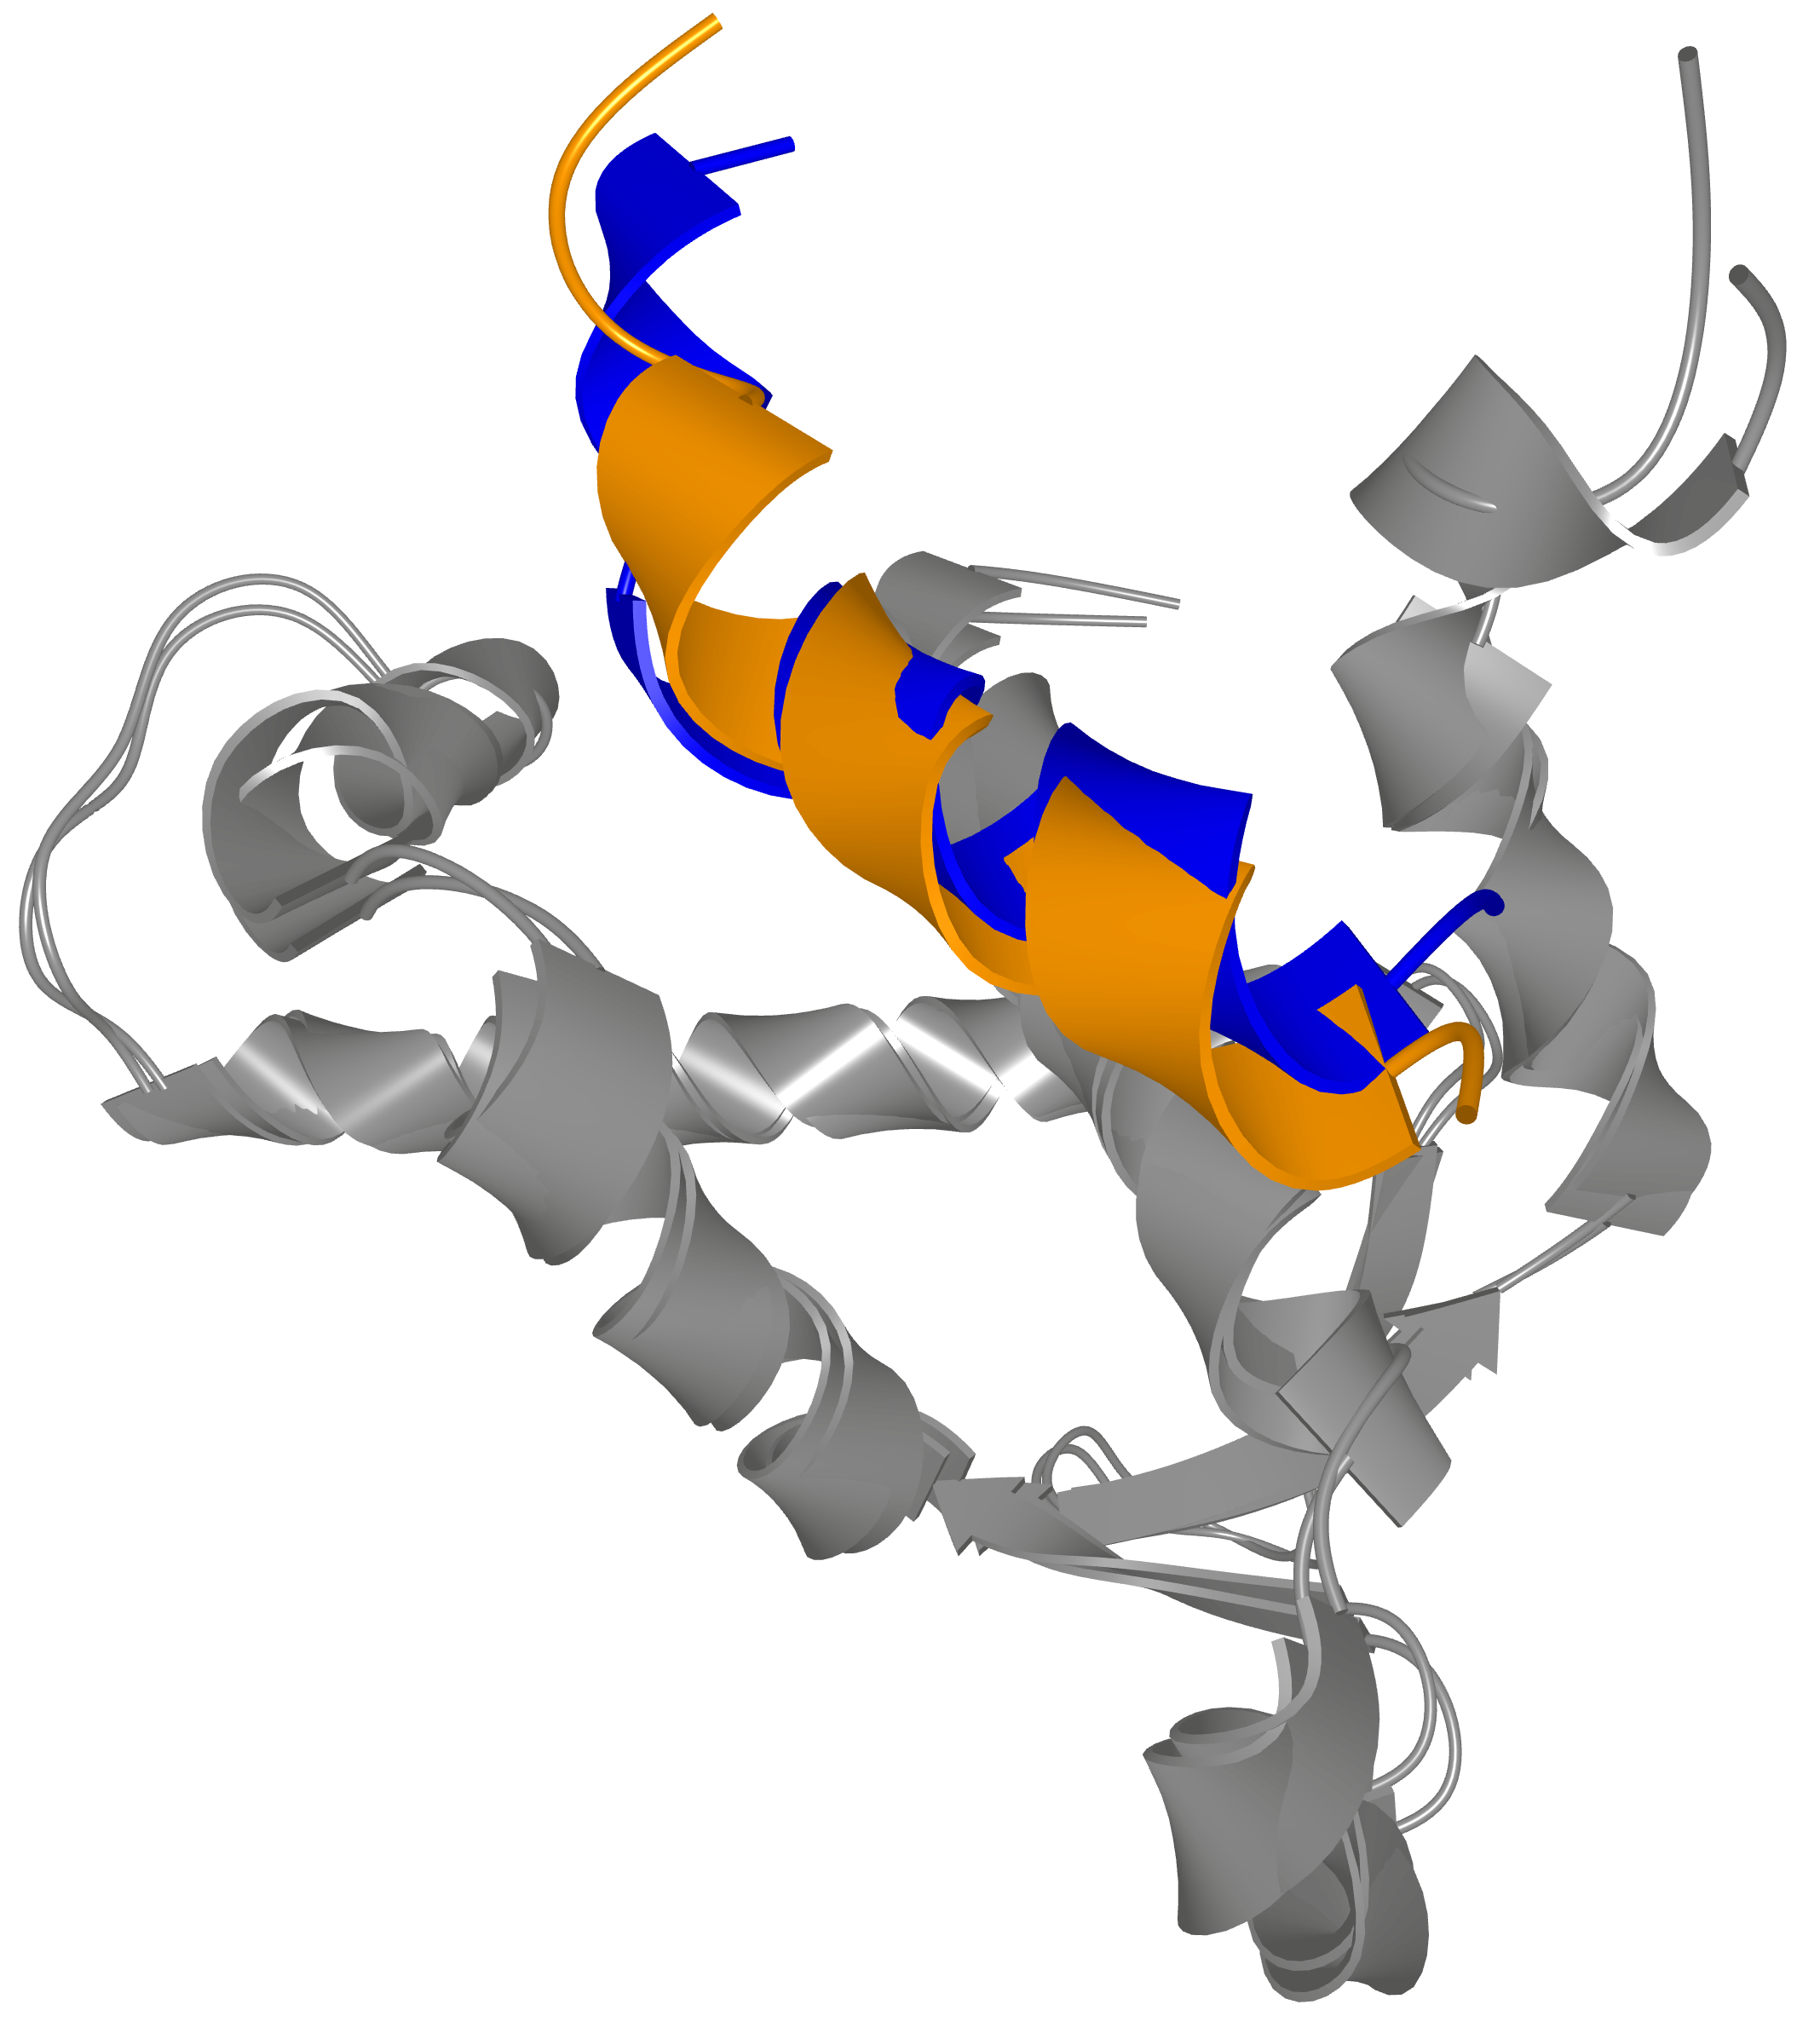
\includegraphics[width=0.9\columnwidth]{images/figure17.png}
  \caption{\csentence{Pocket-String Interaction -- the best fitting HADDOCK configuration.} The best fit HADDOCK configuration (orange) aligned with the 3EUH crystal structure (blue).}
  \label{fig:MukEF_selection_3_best_pair}
\end{figure}

\begin{figure}[h!]
  \centering
  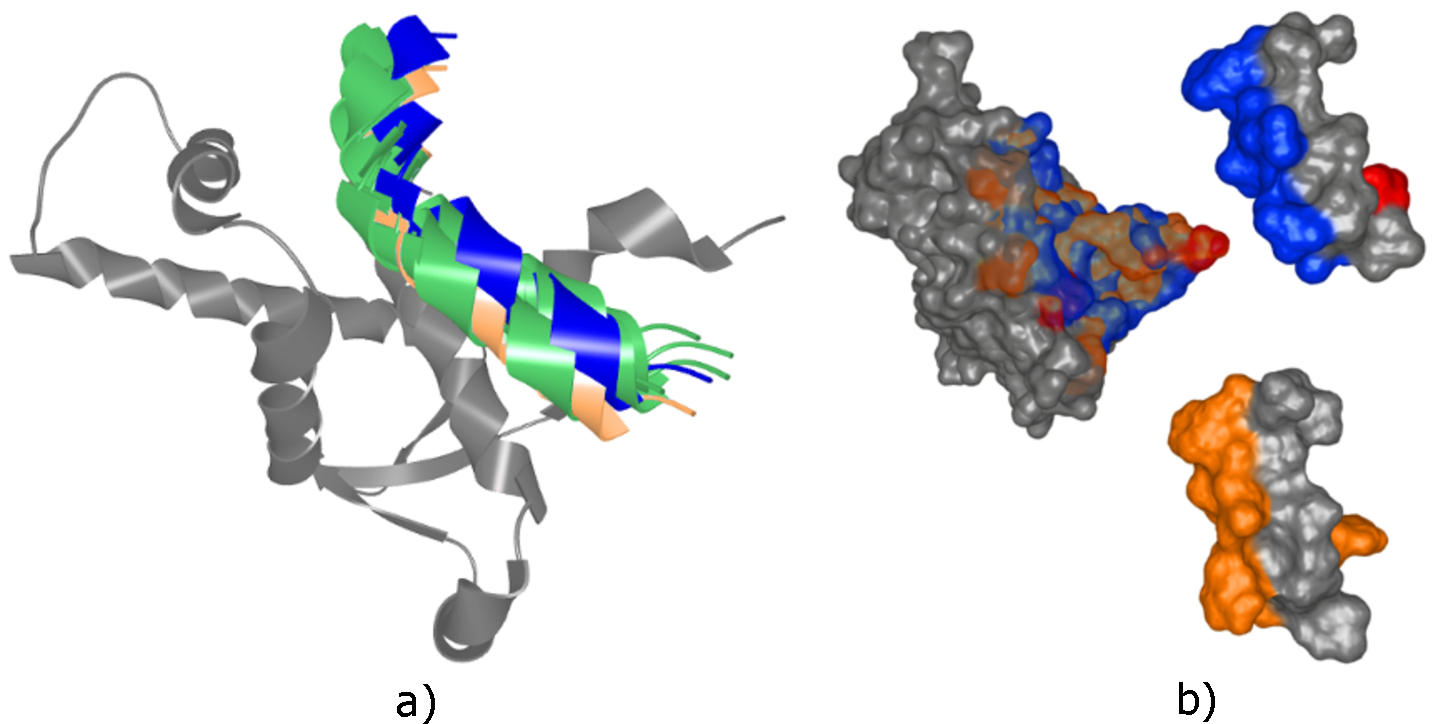
\includegraphics[width=0.9\columnwidth]{images/figure18.pdf}
  \caption{\csentence{\CoZoLists of 3EUH crystal structure computed with different distance parameters.} (a) Contacts computed with the distance parameter 5~\AA. (b) Contacts computed with the distance parameter 4~\AA. The \CoZoLists are sorted according to the distance of the amino acids.}
  \label{fig:list_3euh}
\end{figure}

\begin{figure}[h!]
    \centering 
    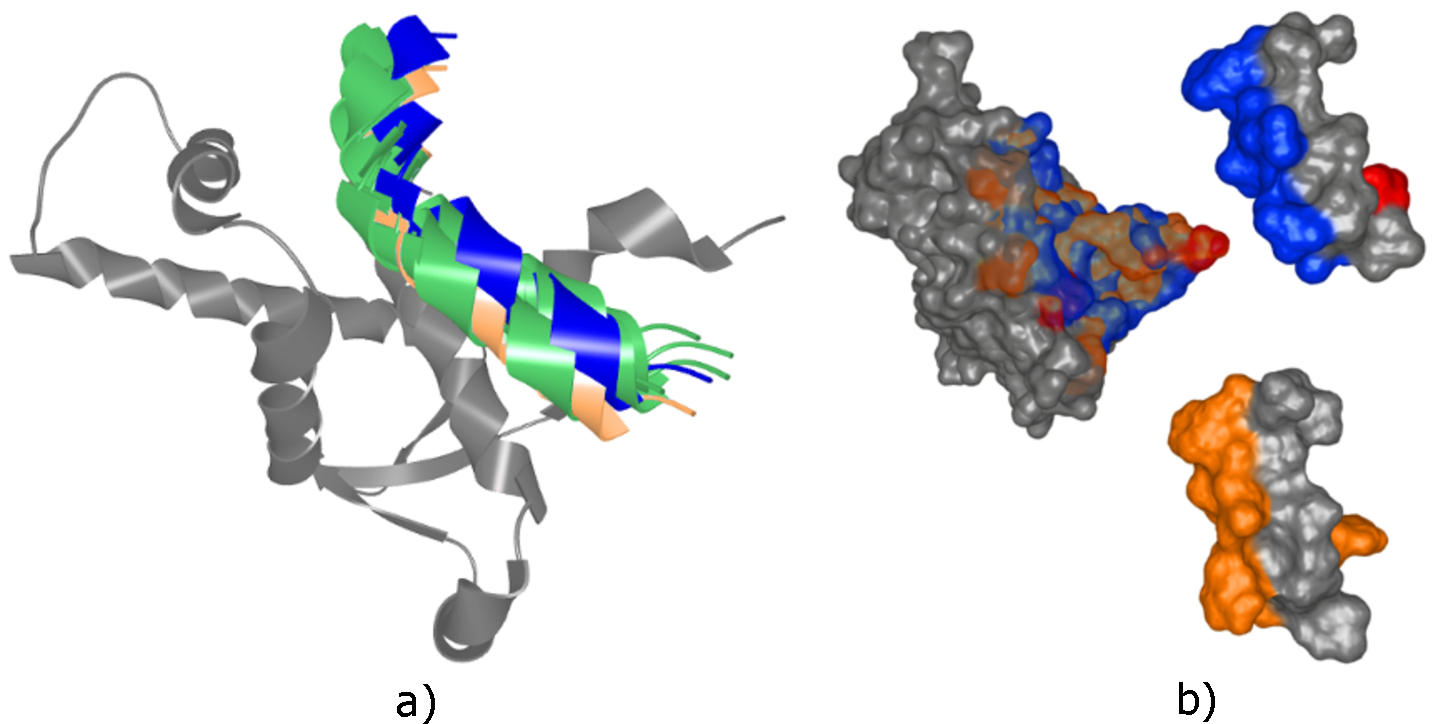
\includegraphics[width=0.9\columnwidth]{images/figure19.pdf}
    \caption{\csentence{Pocket-String Interaction -- the best fitting PyDock configurations.}(a) The best 5 PyDock configurations with the distance parameter 4 \AA,  aligned with the 3EUH crystal structure (blue). The configuration, which exhibited the most similar contacts with the crystal, is orange and the remaining configurations are green. (b) The \ExpView showing the comparison of the contact zones of the best PyDock configuration (orange) with the 3EUH crystal structure (blue).}
  \label{fig:pydock_pocket_string}
\end{figure}



%%%%%%%%%%%%%%%%%%%%%%%%%%%%%%%%%%%
%%                               %%
%% Tables                        %%
%%                               %%
%%%%%%%%%%%%%%%%%%%%%%%%%%%%%%%%%%%

%% Use of \listoftables is discouraged.
%%


%%%%%%%%%%%%%%%%%%%%%%%%%%%%%%%%%%%
%%                               %%
%% Additional Files              %%
%%                               %%
%%%%%%%%%%%%%%%%%%%%%%%%%%%%%%%%%%%

%\section*{Additional Files}
%  \subsection*{Additional file 1 --- Sample additional file title}
%    Additional file descriptions text (including details of how to
%    view the file, if it is in a non-standard format or the file extension).  This might     refer to a multi-page table or a figure.

%  \subsection*{Additional file 2 --- Sample additional file title}
%    Additional file descriptions text.


\end{backmatter}
\end{document}
